\chapter{Top-down Constraints on Atmospheric Mercury Emissions from ASGM Activities}\label{Chapter3}
\section{Background}
\begin{flushleft}


 Numerous prior studies have quantified anthropogenic Hg sources, including ASGM Hg emissions using different methodologies. Bottom-up estimates leverage collected data on underlying activities and emission factors to estimate regional and global totals. For instance, the bottom-up global inventory in the GMA 2018 estimated ASGM Hg emissions to be 838 Mg with an uncertainty range of 675-1000 Mg for 2015 \cite{united_nations_environment_programme_technical_2019,steenhuisen_development_2019}. Moreover, Streets et al. (2019) tested six different proxies for scaling emissions to other years and used an average value to scale the inventory of emissions to the year 2015, thus estimating that ASGM was the largest source and responsible for 775 Mg of emissions\cite{streets_global_2019}. Muntean et al. (2014) also used a bottom-up technique in which they found that poverty in gold ore-rich countries (as measured by the GINI index \cite{sadefo_kamdem_nice_2012}, where available) was correlated with data on ASGM production activity. The poverty-based approach they used estimated that ASGM was responsible for 728.27 Mg emissions in 2010, equivalent to 41.1\% of the global Hg emissions\cite{muntean_evaluating_2018}. Such inventories are essential and a critical input to model Hg using CTMs such as \gc. However, the different assumptions on the activity data and emission factors induce significant uncertainty in the emission inventories. An additional bias in the bottom-up approach originates from the reliance on officially reported emissions data, which might cause differences in accuracy between countries and regions. 
 \end{flushleft}
 \begin{flushleft}
    National baseline Hg-use estimates are bottom-up inventories where countries identify and quantify the sources of Hg released within their borders. Under Article 7 of the MC and Annex C, countries must include in their NAPs baseline estimates of the quantities of mercury used in ASGM within their territory \cite{united_nations_environment_programme_estimating_2017}.  
 \end{flushleft}
 



\begin{flushleft}
On the contrary, top-down emission estimation approaches combine atmospheric transport and chemistry models with atmospheric concentration measurements to quantify emissions. Even though the atmospheric chemistry literature has various top-down method applications, no study explicitly constrains ASGM Hg emissions. For instance, Bousquet et al., 1999 applied top-down methods to infer surface fluxes of atmospheric CO\textsubscript{2} from observed concentrations\cite{bousquet_inverse_1999}. Furthermore, Kopacz et al., 2009, employed top-down techniques to quantify source contributions to ozone pollution at two adjacent sites on the U.S. west coast in the spring of 2006\cite{kopacz_global_2010}. They used  \gc as a common intercomparison platform to show global consistency between the satellite data sets and the in situ data. This underscores the role models such as GEOS-chem have as integration platforms for differently sourced data to generate unified insights. Likewise, Hg emissions have been constrained using top-down methods in Song et al., 2015 where a top-down approach at a global scale is applied to quantitatively estimate present-day Hg emission sources and critical parameters in GEOS-Chem to better constrain the global biogeochemical cycle of Hg\cite{song_top-down_2015}. Moreover, Denzler et al., 2017 used a top-down approach to quantify Hg emissions on a European scale based on the atmospheric Hg measurements conducted at the remote high-altitude monitoring station, Jungfraujoch, Switzerland\cite{denzler_inversion_2017}. 
\end{flushleft}
\begin{flushleft}
In this chapter, I apply a top-down approach at a regional scale to estimate ASGM Hg emissions (emission inversion) from Peru. Until now, no scientific studies have provided top-down constraints for ASGM emissions using atmospheric transport models and Hg atmospheric monitoring data. Section 3.2 describes the overall methodology. I combine ground-based observations of atmospheric Hg from the case study region\cite{koenig_seasonal_2021}, a national inventory for Peru\cite{artisanal_gold_council_reporte_2017} and simulations with the GEOS-Chem global CTM. Reference (also known as a priori) emissions are from the GMA 2018\cite{steenhuisen_development_2019,united_nations_environment_programme_technical_2019}. The Markov Chain Monte Carlo is the inversion method used (Sect. 3.2.2) to obtain the optimized (a posteriori) emissions, considering uncertainties associated with reference and ground-based observations. Section 3.3 presents results and discussion. Comparisons of observations and model outputs are given in Sect. 3.3.1. The optimized emissions from 5 regions in Peru are shown in Sect. 3.3.2. Finally, I discuss the implications of the inversion results for providing baseline estimates of ASGM Hg emissions  and summarize my conclusions (Sect. 3.3.4).

\end{flushleft}
\newpage
\section{Methods}
\begin{flushleft}
    In the results section of chapter 2 of this thesis, I discussed the differences between the \gc model predictions of Hg at various measuring stations and in Latin America. One of the hypotheses proposed attributed the differences between the model and the observations to how the emissions were parameterized in \gc. The input emissions in \gc are determined by the Hg inventory; hence, I first evaluated the Hg inventory used in the model against other global inventories. Next, the inventory was compared to a national inventory for Peru \cite{agc_reporte_2017}. Once the differences between the global inventory\cite{steenhuisen_development_2019} and the Peruvian national inventory were analyzed, the global inventory was re-gridded to the GEOS-Chem grid, and the emissions from grid boxes corresponding to different departments in Peru were scaled. The scaled inventories were used to create the simulations described in Table \ref{tab:all_geos_chem_simulations}. These simulations were used to determine the sensitivity of the Hg concentration at distant locations to the changes in emissions from the grid boxes in the case study region. The simulated \hgc in the atmosphere was compared to the observed TGM concentration in the atmosphere to determine the sensitivity of the \hgc to the changes in emissions from individual grid boxes and multiple grid boxes. 
\end{flushleft}

\subsection{Mercury Emission Inventories}
\begin{flushleft}


Globally gridded emissions inventories such as those shown in Figure \ref{fig:Hg_inventories} are a critical input to CTMs such as\gc. Figure \ref{fig:Hg_inventories} shows the distribution of Peruvian anthropogenic Hg emission estimates by different global inventories \cite{united_nations_environment_programme_technical_2019,steenhuisen_development_2019,muntean_evaluating_2018,streets_global_2019}. The plot on the right shows how anthropogenic Hg emissions were distributed in the  Streets et al. 2019 Hg emissions inventory\cite{streets_global_2019}. They analyzed the global and regional trends in anthropogenic Hg releases to the atmosphere between 2010 and 2015 and the associated trends in modeled and measured Hg concentrations at sites around the world. Their Peru total Hg emissions estimate was about 40 tonnes per year. The plot in the middle shows how anthropogenic Hg emissions were distributed in the EDGAR ASGM Hg emissions inventory\cite{muntean_evaluating_2018}. This global mercury emissions inventory includes emissions from all key mercury emitting sources, and Peru's total Hg emissions estimate was about 26 tonnes per year. Finally, the GMA 2018 ASGM Hg emissions estimates for 2015 are shown on the right. The Hg emissions were distributed by assigning emission estimates to geo-located point sources, using reported emissions information where available, and otherwise assigning a modeled emission to the point. Emissions that could not be assigned to point sources were distributed using sector-specific proxies. The ASGM proxies for ASGM Hg emissions in Peru were the locations of legal mining concessions and the global alluvial gold map. This inventory estimated that ASGM was responsible for about 110 tonnes of annual emissions in Peru. The GMA 2018 inventory is used in all the GEOS-Chem simulations conducted in this study. This inventory was used because it was more representative of the ASGM emissions than the other two inventories, as the total Hg emissions are compatible with bottom-up baseline ASGM Hg emissions. ASGM emissions in this inventory were distributed based on a system that uses a probability approach to estimate ASGM activity and then distributes the emission estimate according to that probability\cite{steenhuisen_development_2019}. The global alluvial gold map and a (gold) mining concessions  \href{(https://data.globalforestwatch.org/search?collection=Dataset&q=mining)}{data set} were used to distribute ASGM emissions for Peru. 
\end{flushleft}
\begin{figure}[H]
  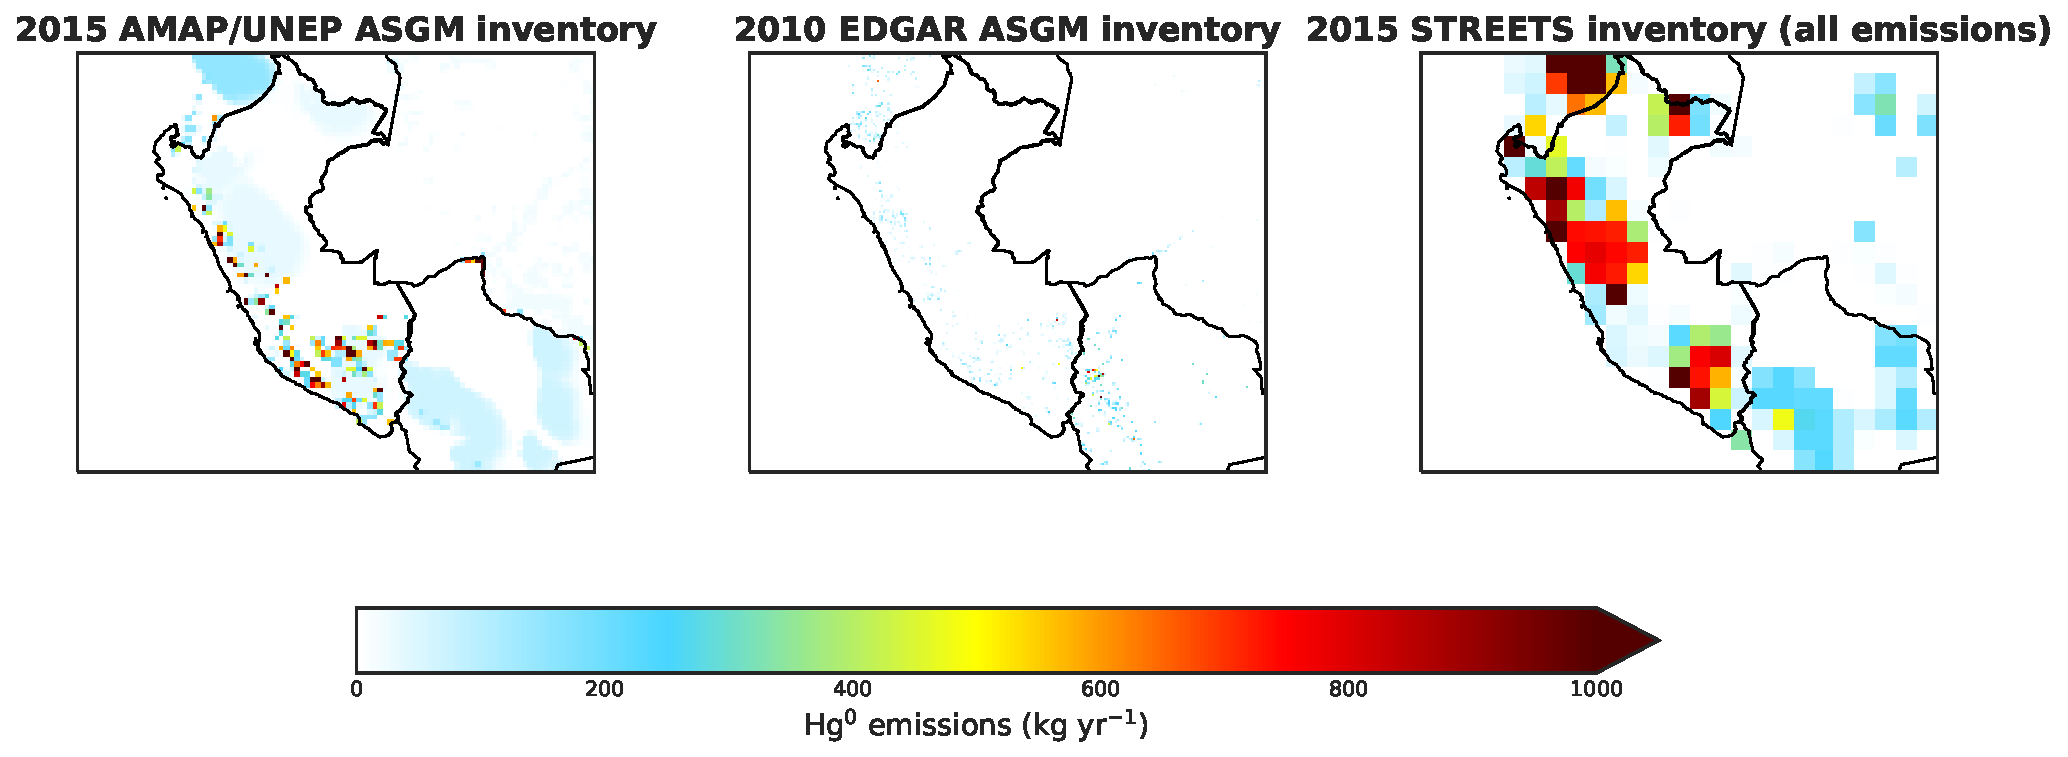
\includegraphics[width=\textwidth]{templates/figures/Peru_Maps/Hg_inventories.pdf}
  \centering
  \caption{Comparison of Hg emission from Peru as estimated by different global inventories \cite{united_nations_environment_programme_technical_2019,steenhuisen_development_2019,muntean_evaluating_2018,streets_global_2019}.}
  \label{fig:Hg_inventories}
\end{figure}
\FloatBarrier


\subsection{Emission Modification and \gc Simulations}
\begin{flushleft}
    Five more simulations were added to the \on and \off \gc simulations presented in Chapter 2. The other five simulations were sensitivity runs that used modified emission inventories corresponding to changes in emissions from one of the grid boxes in the case study region.
\begin{figure}[H]
\centering

\begin{tabular}[H]{c}

\subfloat[GMA 2015 Grid]{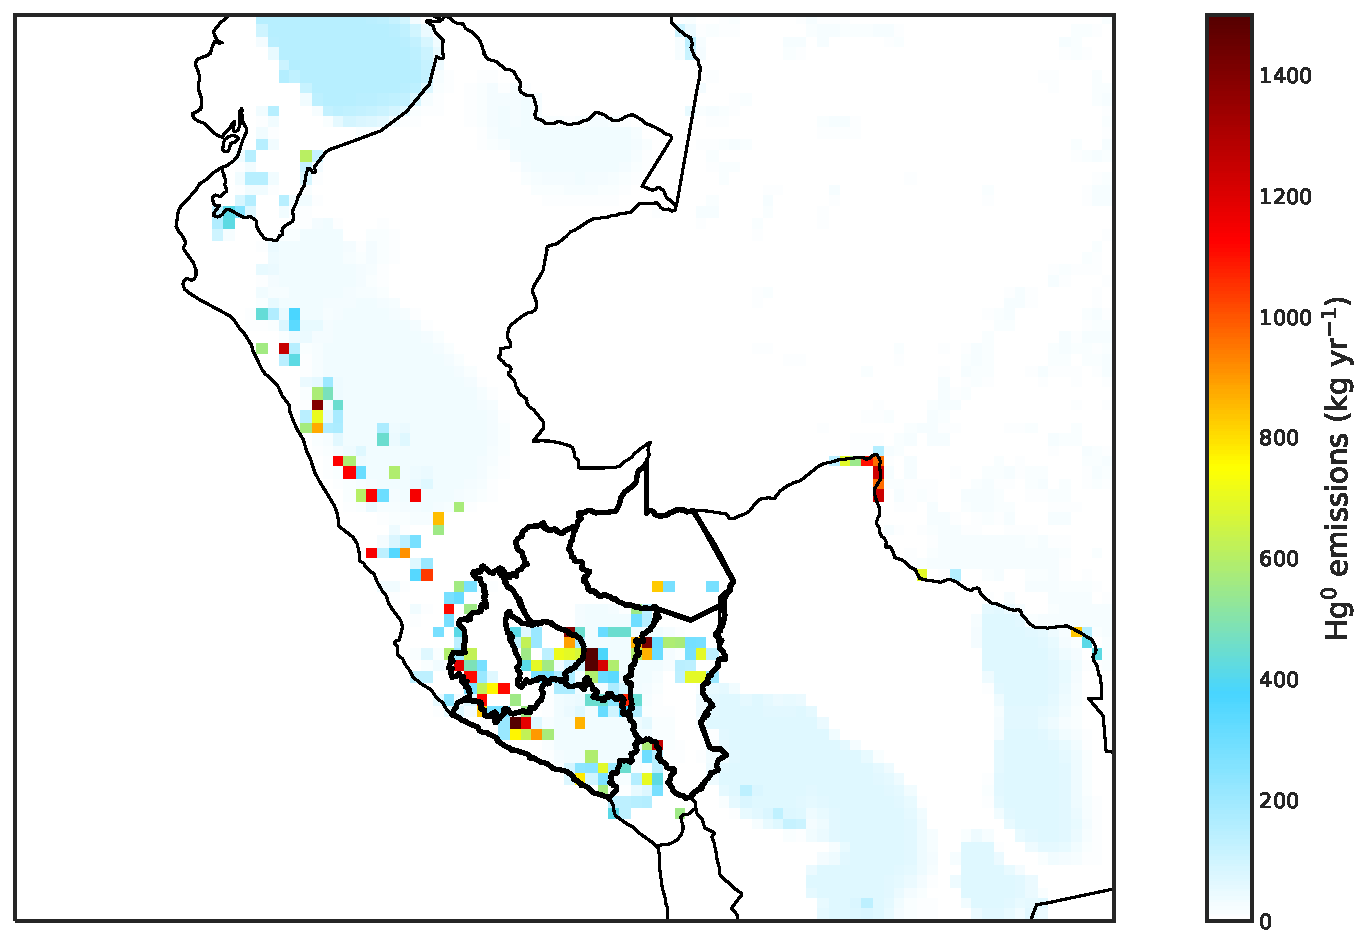
\includegraphics[width = 0.8\linewidth]{templates/figures/Peru_Maps/GMA2018inventory025x025.pdf}}\\
\subfloat[GEOS Chem Grid]{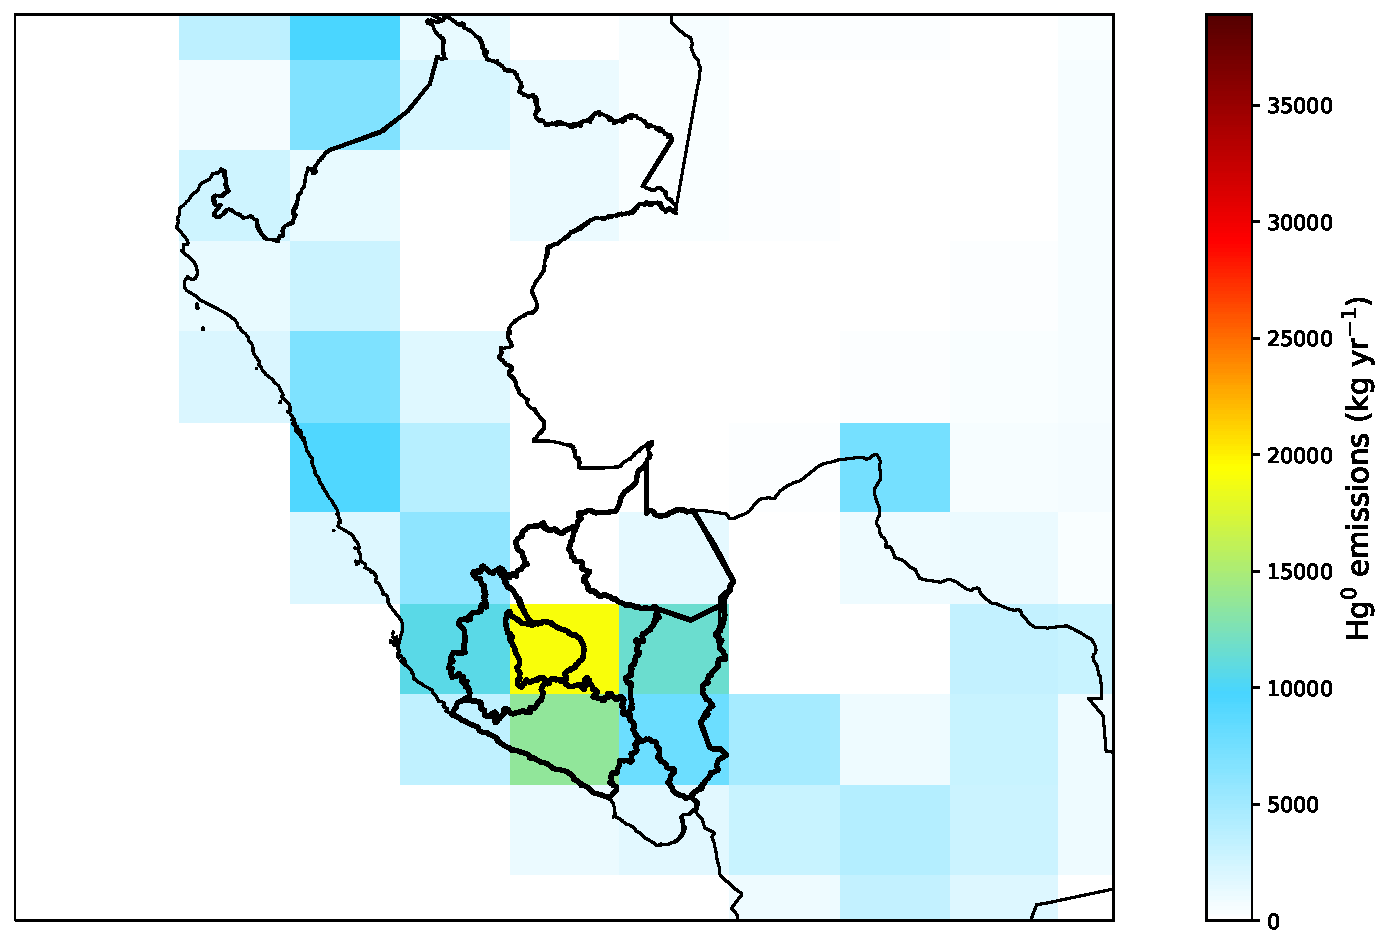
\includegraphics[width = 0.8\linewidth]{templates/figures/Peru_Maps/GMA2018inventory2x25.pdf}}


\end{tabular}
  

\captionof{figure}{Maps showing how the GMA2018 emission estimates for the year 2015 were distributed for Peru before re-griding (a) and after re-gridding to the \gc grid (b) }
\label{fig:GMA2018}
\end{figure}
\FloatBarrier
\end{flushleft}


\begin{table}[H]
\caption{Table showing the different GEOS-Chem simulations used in the analysis}
    \label{tab:all_geos_chem_simulations}
\begin{tabular}{lcp{0.5\linewidth}}

\textbf{Simulation Name}    &  Resolution       & \textbf{Description Estimate}                             \\
\hline
Base (ASGM=ON)              & 2.0$\times$2.5        & All Hg anthropogenic emission sources are turned on  \\
No ASGM (ASGM=OFF)          & 2.0$\times$2.5        & All ASGM emissions are turned off                     \\
Mdd                         & 2.0$\times$2.5        & Emissions from the \gc grid box located in  Madre de Dios  were scaled up by a factor of 2 \\

Apr                         & 2.0$\times$2.5        & Emissions from the \gc grid box located in Apurimac were scaled down by a factor of 0.5\\

Aqp                         & 2.0$\times$2.5        & Emissions from the \gc grid box located in Arequipa department were scaled up by a factor of 2\\

Npun                        & 2.0$\times$2.5        & Emissions from the \gc grid box located in the northern region of Puno were scaled up by a factor of 2 \\

Spun                        & 2.0$\times$2.5        & Emissions from the \gc grid box located in the southern region of the Puno were scaled up by a factor of 2 \\
\hline
\end{tabular}
\centering
\end{table}

\newpage
\subsection{Simulated Atmospheric Mercury Concentration Signals}
\begin{flushleft}
The relationship between the \hg emissions from a specific grid box and the \gc simulated atmospheric \hg concentration at distant points from the emissions source is assumed to be defined by a linear function. This means that an increase in emissions is expected to increase the \hg concentration. Consequently, the relationship between emissions and concentrations can be represented by the following equation:


\begin{equation}
\label{doublingSig}
Hg^0_{sig(region)}=Hg_{m_0}+\small\frac{(Hg_{m_1} -Hg_{m_0})}{(m_1 -m_0)}(m_{(region)} -m_0)
\end{equation}
where:
\end{flushleft}

\begin{description}[leftmargin=!,labelwidth={5 em}]
    \item [$region$] is the location of the emission source within the case study region.
    \item [$Hg^0_{sig(region)}$] is the simulated \hg concentration at the observation site due to $m_{(region)}$ at the grid box in the specific $region $ of interest.
    \item [$Hg_{m_0}$] is the Hg concentration  at the observation site generated by the Base (ASGM =ON) simulation. 
    \item [$Hg_{m_1}$] is the Hg concentration  at the observation site generated by the $i^{th}$ region simulation $i$=Mdd,Apr, Aqp,Npun,Spun. 
    \item [$m_1$] is the amount of emissions in Mega grams after scaling the emissions from a specific grid box.
    \item [$m_0$] is the amount of emissions in Mega grams before scaling the emissions from a specific grid box.
\end{description}


% \begin{flushleft}
% $Hg_{sig(region)}$ gives the Hg concentration signal in the atmosphere that results from a unit change in the tonnes of emissions from a specific grid box. Therefore, $Hg_{sig(region)}$ was used to investigate the sensitivity of the observations to the different amounts of additional ASGM Hg emissions and the regional grid boxes. The Hg concentration in the atmosphere that results from a specific change in emissions from a particular grid box was calculated using Equation \ref{ysignal} below.
% \begin{equation}
% \label{ysignal}
% \small{Hg_{m(region)}} =Hg_{sig(region)}(m-m_o), 
% \end{equation}
% where:
% \end{flushleft}


% \begin{description}[leftmargin=!,labelwidth={1.5 em}]
    
%     \item [$m_0$] is the GMA 2018 ASGM emissions estimate in metric tonnes for the particular grid box corresponding to a place in the case study region
    
%     \item [$m$] is the amount of emissions, in metric tonnes, from a grid box required to produce $Hg_{m}$ concentration in the atmosphere
% \end{description}




% \begin{flushleft}
% For each grid box in the case study region, the emissions were modified from their original GMA 2018 estimates to new values based on Hg emission estimates produced by the Artisanal Gold Council(AGC)
% \end{flushleft}

\subsection{Observation Site Selection}

\begin{flushleft}
TGM and GEM observation data from different locations in Latin America were analyzed and compared to the \gc simulated \hg concentrations for those sites in Chapter 2. The \gc predictions for ASGM contributions to atmospheric Hg concentration were higher at the CHC, making it an excellent candidate to use as a reference for comparison with the modified \gc Hg concentration predictions. Moreover, this site is the closest monitoring site to Peru hence it is expected that it would be more likely to detect atmospheric \hg changes that result from the changes in Hg emissions from the case study region. The time series of the observed concentration at the CHC station between July 2014 and January 2016 is shown in Figure \ref{fig:chc_time_series}.
\end{flushleft}

\begin{figure}[H]
  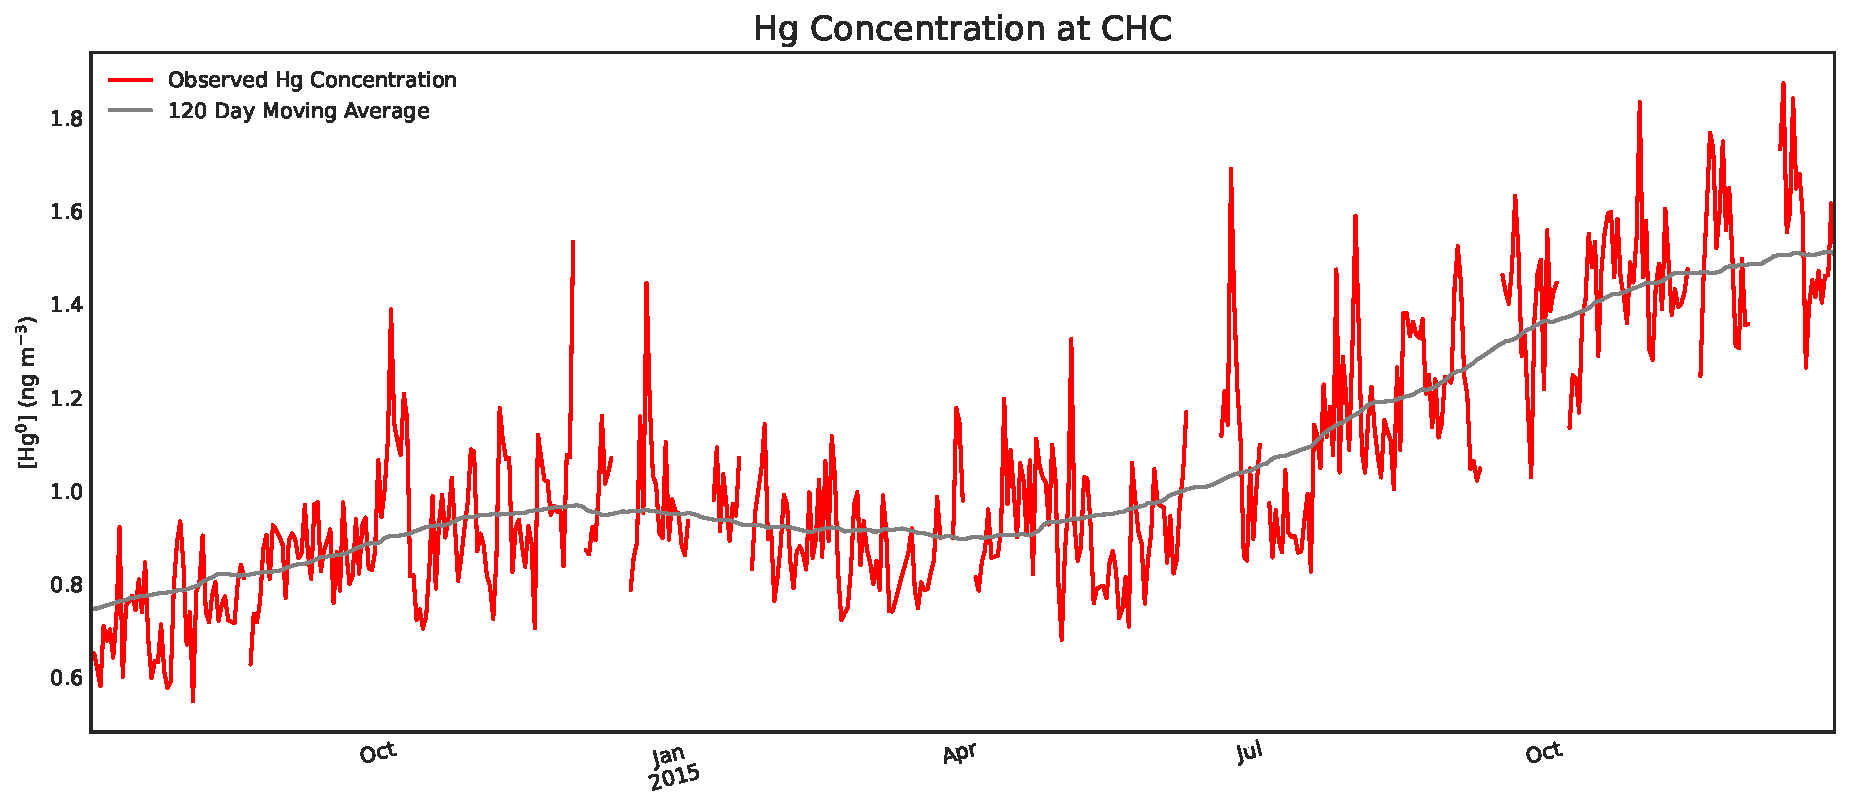
\includegraphics[width=\textwidth]{templates/figures/GMOS_Sites/ObsTimeSeries.pdf}
 
  \caption{The average daily TGM concentration at CHC in ng m\textsuperscript{-3} as a function of time over the measurement period from July 2014 to January 2016. The daily average concentration is indicated by the red line, while the grey line shows the 120-day moving average, which highlights the upward trend in the daily averages}
  \label{fig:chc_time_series}
  \centering
\end{figure}
\FloatBarrier
\begin{flushleft}

The detailed characteristics of the observations over this measurement period were described in Koenig et al. (2020); hence our analysis focused on using the observation TGM data to evaluate the performance of the GEOS-Chem model in predicting the \hg based on the input \hg emission inventories. As shown in Figure \ref{fig:chc_time_series}, the TGM concentration at CHC showed an upward trend, which Koenig et al. (2021) attribute to El Ni\~no-Southern Oscillation (ENSO)\cite{koenig_seasonal_2021}. As a result, they categorized the measured TGM concentrations in the atmosphere at the CHC site as normal conditions (NC), 2014-07 to 2015-05, and ENSO conditions from 2015-06 to 2016-01. To reduce the number of records associated with ENSO, I limited my analysis to one year's worth of data from 2014-07 to 2015-07.
\end{flushleft}

\subsection{ Inverse Modelling with Markov Chain Monte Carlo}
\begin{flushleft}
    Inverse modeling is described by Brasseur, and Jacob \cite{brasseur_modeling_2017} as a method for quantifying variables that drive a physical system using observations. Accordingly, the variables are statistically optimized based on the observational and other information available. Variables we wish to optimize are called state variables and assembled into a state vector $x$. In the same way, the observations are assembled into an observation vector $y$. The forward model $F$ of the physical system describes the relationship between $x$ and $y$:

    \begin{equation}
\label{inverse_model}
y=F(x,p) + \epsilon_0
\end{equation}
where:\\
\begin{description}[leftmargin=!,labelwidth={3 em}]
    \item [$p$] contains all variables in the model that we will not optimize as part of the inversion
    \item [$\epsilon_0$] a vector of observations errors, which includes errors from measurements, the forward model, and model parameters 
\end{description}
 Forward models describe the effects of the system as functions of the cause $x$, usually by using equations that describe the system's physics. The cause ($x$) can be quantified via inversion of the model based on the effect ($y$). Moreover, $x$ is estimated with some statistical error when $\epsilon_0 \neq 0$ is present. The solution for $x$ is called the optimal estimate, posterior estimate, or retrieval. \cite{brasseur_modeling_2017}. 
 \end{flushleft}

\begin{flushleft}
    The uncertainty in obtaining $x$ from $y$ requires us to consider constraints on the value of $x$ called priors that could reduce the error on the optimal estimate.  We generally use the prior estimate $x_A$ as a constraint, representing our best estimate of $x$ before the observations. It has some error $\epsilon_A$. As a result, the ideal estimate must consider the relative information given by the observations $y$ and the prior estimate $x_A$. The error statistics of the estimates $\epsilon_O$ and $\epsilon_A$. We can analyze the relative importance of observations and prior knowledge by using inverse modeling. In this way, it provides insight into the effectiveness of an observing system in constraining $x$\cite{brasseur_modeling_2017}.

    \end{flushleft}

\begin{flushleft}
For this analysis, we use the measured Hg concentration (observation vector $y$) to constrain the  emissions from grid boxes in the case study region (state vector $x$). The forward model is given by the linear combination of the signals generated by the GEOS-Chem model as shown in Equation \ref{Hg_conc} below:

\begin{align}
\begin{split}\label{Hg_conc}
Hg_{conc}= {}&Hg_{m(MdD)}+ Hg_{m(S-Puno)} + Hg_{m(N-Puno)} + Hg_{m(Apr)}+ Hg_{m(Aqp)}\\
            & +Hg_{m_0}
\end{split}
\end{align}

where:
\end{flushleft}

\begin{description}[leftmargin=!,labelwidth={5 em}]
    \item [$Hg_{m(MdD)}$] is the Hg concentration signal resulting from emissions from the Madre de Dios (MdD) grid box
    \item [$Hg_{m(S-Puno)}$] is the Hg concentration signal resulting from emissions from the South Puno (S-Puno) grid box
    \item [$Hg_{m(N-Puno)}$] is the Hg concentration signal resulting from emissions from the North Puno (N-Puno) grid box
    \item [$Hg_{m(Apr)}$] is the Hg concentration signal resulting from emissions from the Apurimac (Apr) grid box
    \item [$Hg_{m(Aqp)}$] is the Hg concentration signal resulting from emissions from the Arequipa (Aqp) grid box
    \item [$Hg_{m_0}$] is the baseline Hg concentration signal.
\end{description}

\begin{flushleft}
Each of the $Hg_{m(region)}$ terms of Equation \ref{Hg_conc} represent signals from the different departments are calculated using Equation~\ref{doublingSig} an the form the parameter vector $p$. The $m_{(region)}$ terms are the only unknowns and the equation can be expanded to isolate the terms with $m_{(region)}$, which is the parameter we are optimizing for in the inverse modeling method. The expanded form of Equation \ref{Hg_conc} is shown below:

\begin{align}
\begin{split}\label{Hg_cons_expanded_form}
Hg_{conc}={}& (m_{(MdD)}Hg_{sig_{(MdD)}} -m_oHg_{sig_{(MdD)}})+ (m_{(S-Puno)}Hg_{sig_{(S-Puno)}} -m_oHg_{sig_{(S-Puno)}}) \\
            &+ (m_{(N-Puno)}Hg_{sig_{(N-Puno)}} -m_0Hg_{sig_{(N-Puno)}}) + (m_{(Apr)}Hg_{sig_{(Apr)}} -m_oHg_{sig_{(Apr)}}) \\
            &+ (m_{(Aqp)}Hg_{sig_{(Aqp)}} -m_oHg_{sig_{(Aqp)}})+Hg_{m_0}
\end{split}
\end{align}

Since the values of $m_{(region)}$ are the state variable we want to estimate, they can be represented as $\theta_i=m_{(region)}, i=1$ and the other terms, including the background concentration, are combined into one constant, C:

\begin{equation}
\begin{aligned}
    Hg_{conc}  & = \theta_0C  + \theta_1Hg_{sig_{(MdD)}}+ \theta_2Hg_{sig_{(S-Puno)}} +  \theta_3Hg_{sig_{(N-Puno)}} \\
                & \ \ \ \  +\theta_4Hg_{sig_{(Apr)}} +  \theta_5Hg_{sig_{(Aqp)}}
\end{aligned}
\end{equation}

\begin{align}
Hg_{conc} =\begin{bmatrix} C & Hg_{sig_{(MdD)}} & Hg_{sig_{(S-Puno)}} &Hg_{sig_{(N-Puno)}} &Hg_{sig_{(Apr)}} &Hg_{sig_{(Aqp)}}\end{bmatrix} \times 
            \begin{bmatrix} \theta_0 \\ \theta_1 \\ \theta_2\\ \theta_3\\ \theta_4\\ \theta_5  \end{bmatrix}
\end{align}
where $\theta_0=1$ and $Hg_{conc}$ is the modeled Hg concentration at the observation site of interest.
\end{flushleft}


\begin{flushleft}
The Markov-Chain Monte Carlo (MCMC) is a valuable sampling method for fitting models to data\cite{hogg_data_2018}. We apply the MCMC to constrain ASGM Hg emissions from the case study region in Peru.  The model is generated by a set of parameters and emissions, and we aim to sample from the parameters that best fit our data. The MCMC compares the modeled concentrations to the observed data using metrics such as the \nft confidence interval, mean, and the \iq. The MCMC models given data by sampling around optimum values from the posterior distribution. The MCMC is a Bayesian approach; hence it requires the definition of priors on the parameters of interest. The priors encode information that we already know of the system. The probability of the model given the observed data is given by the posterior probability, $P(\theta|D)$, which is calculated using the Bayes theorem:

\begin{equation}
\label{bayes_eq}
P(\theta|D)=\frac{P(D|\theta)P(\theta)}{P(D)}
\end{equation}
where:
\end{flushleft}

% \begin{description}[leftmargin=!,labelwidth={3 em}]
%     \item [$P(D|\theta)$] is the likelihood which is the probability of the data given the model
%     \item [$P(\theta)$] is the prior, which is the probability of the model and 
%     \item [$P(D)$] is the evidence which is the probability of the data.
% \end{description}

\begin{flushleft}
The MCMC enables the estimation of the sampling of the posterior distribution, which is the left-hand side of Equation~\ref{bayes_eq}. The MCMC is set up by following a set of steps that include defining a function that outputs a model given a set of input parameters and establishing an ensemble of walkers defined by a $\theta$ vector that contains a set of parameters from the model generating function.
Next, the metrics being compared to their observed counterparts are calculated to be used in Equation \ref{model_definition} during the MCMC simulation. 
\end{flushleft}

% \begin{align}
% \begin{split}\label{model_definition}
% \hat{y}= {}&Hg_{m(MdD)}+ 
% \end{split}
% \end{align}


\newpage
\section{Results and Discussion}
\subsection{National vs. Global Mercury Inventory}
Figure \ref{fig:agc_vs_gma18} compares ASGM Hg emissions estimates from two different bottom-up inventories regrided to the GEOS-Chem 2$\times$2.5 grid used in the simulations in this study. The GMA 2018  estimates of Hg emissions from ASGM activities in Peru for 2015 as distributed by Steenhuisen and Wilson\cite{steenhuisen_development_2019} are shown in Figure \ref{fig:agc_vs_gma18},(a). Furthermore, Figure \ref{fig:agc_vs_gma18},(b) represents my interpretation of how the Peru ASGM Hg emissions estimates from the Artisanal Gold Council's(AGC) inventory\cite{agc_reporte_2017} would be mapped on to the GEOS Chem Grid. The estimates for the total ASGM emissions from Peru are almost similar in both inventories, 110.4 t/y in the GMA 2018 and 108.74 t/y in the AGC national inventory.

% \begin{figure}[H]
% \centering

% \begin{tabular}[H]{cc}

% \subfloat[]{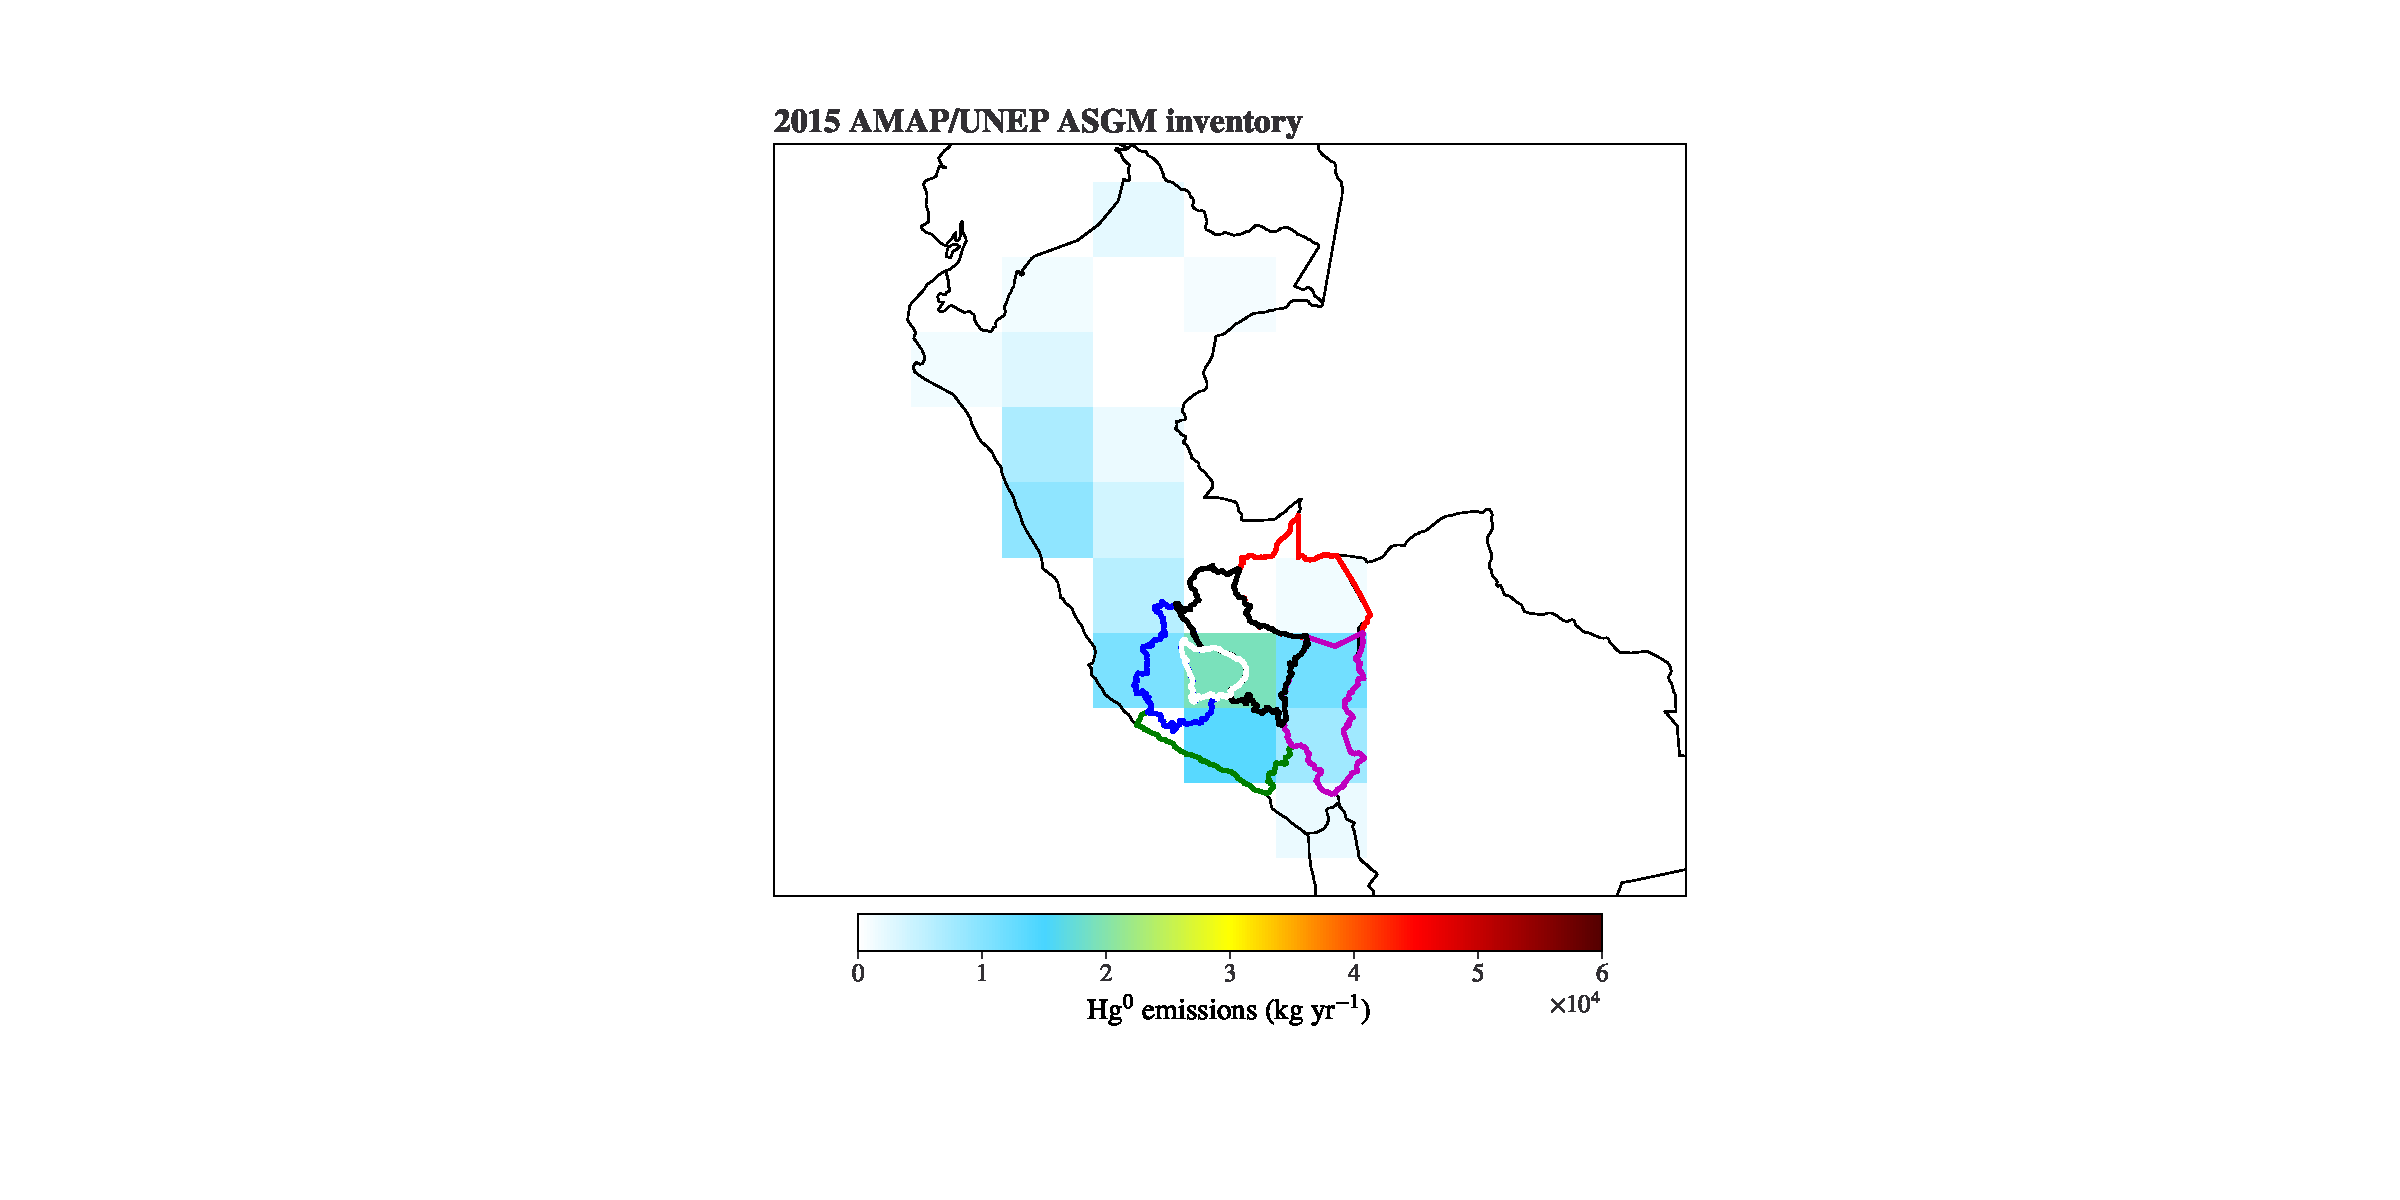
\includegraphics[width = 0.5\linewidth]{templates/figures/Peru_Maps/GMA2018inventory2x25Peru.pdf}}
% \subfloat[]{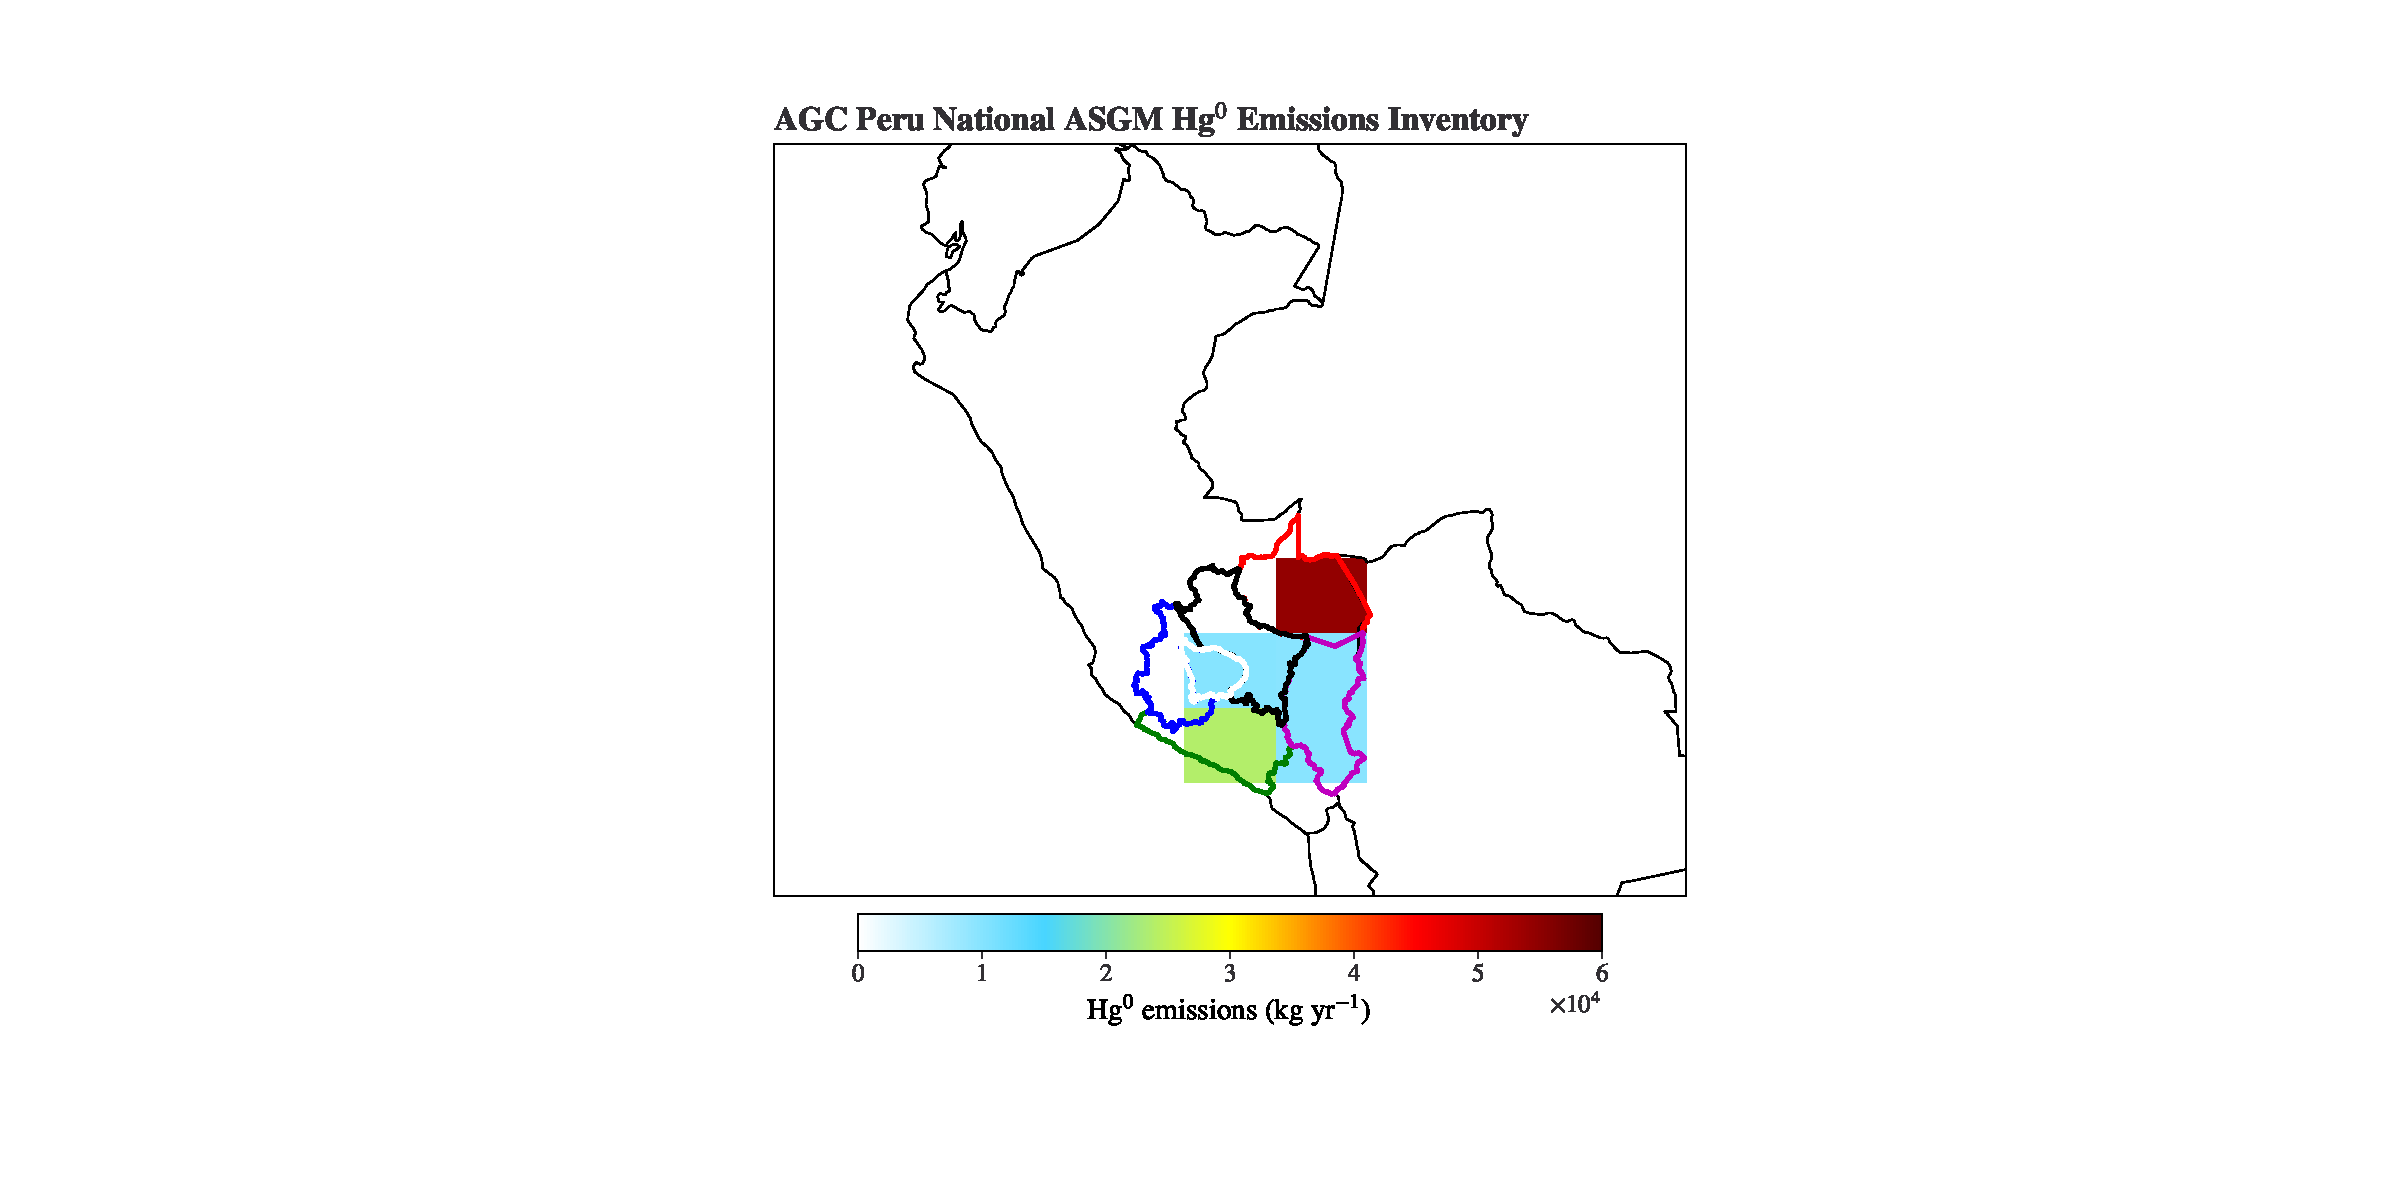
\includegraphics[width = 0.5\linewidth]{templates/figures/Peru_Maps/AGCinventory2x25Peru.pdf}}\\


% \end{tabular}
\begin{figure}[H]
\centering
  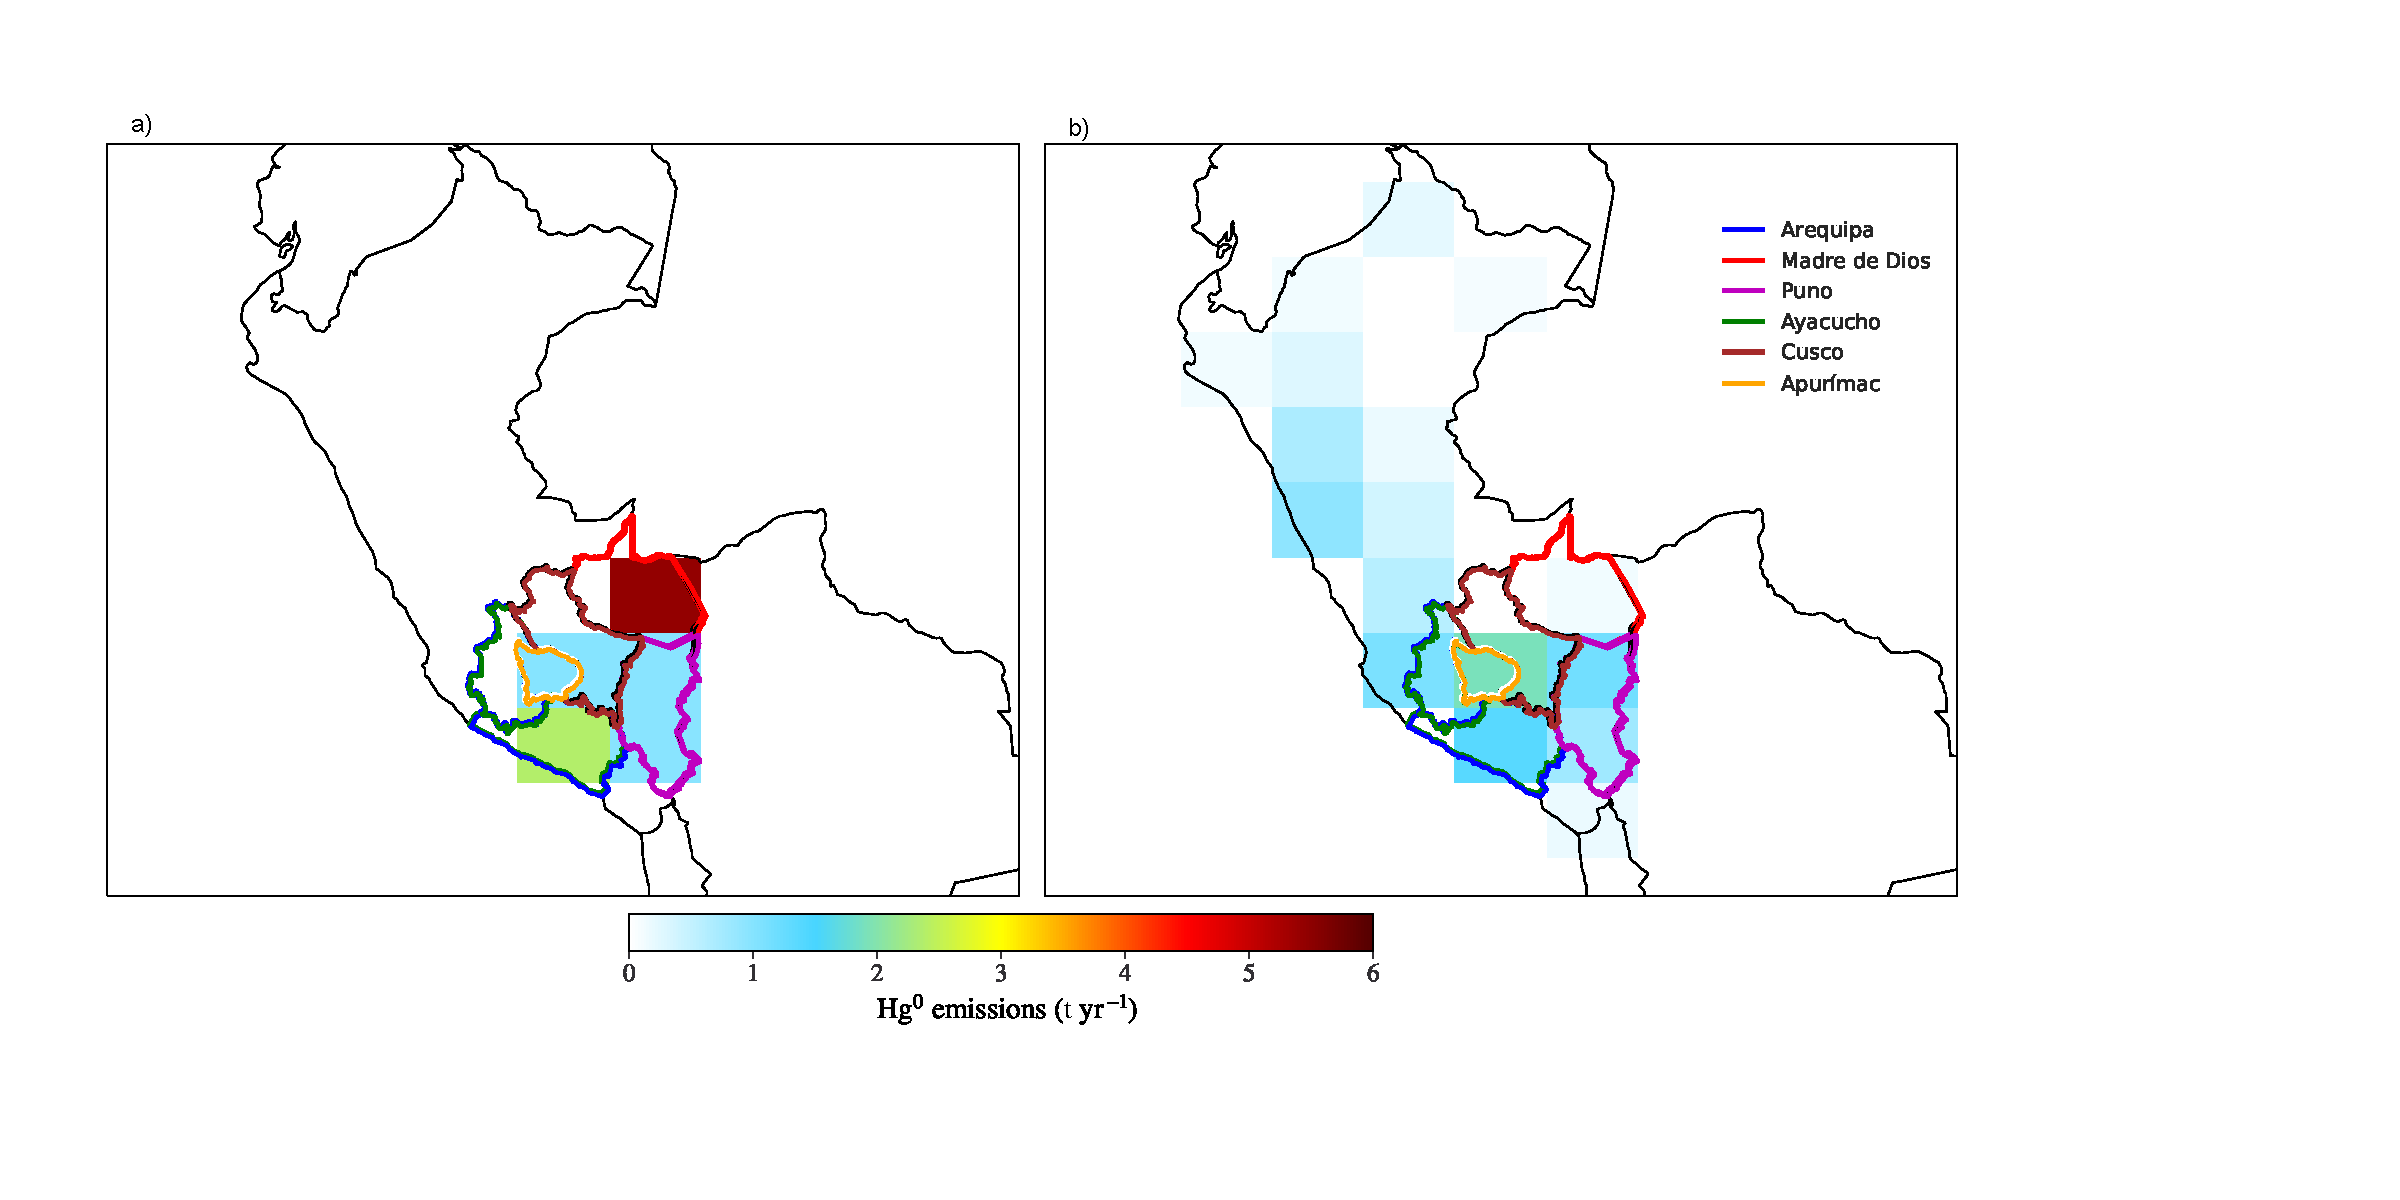
\includegraphics[width=\textwidth]{templates/figures/Peru_Maps/comparison_AGC_GMA18.pdf}  

\captionof{figure}{The AGC Peru National ASGM Hg emissions inventory as published in \cite{agc_reporte_2017} and regridded to the GEOS-Chem 2$\times$2.5 grid resolution is shown in (a).How the ASGM Hg emissions in Peru were distributed in two bottom-up inventories. The GMA2018 ASGM Hg emissions inventory for 2015 as distributed in \cite{steenhuisen_development_2019} and regridded  to the GEOS-Chem 2$\times$2.5 grid resolution is shown in (b).}
\label{fig:agc_vs_gma18}
\end{figure}
\FloatBarrier
\begin{flushleft}
The AGC's Peru national inventory attributed most of the ASGM Hg emissions to the South Eastern departments in the country\cite{agc_reporte_2017}. As seen in Table\ref{tab:agc_vs_gma18}, the Madre de Dios department is the largest source of Hg emissions, followed by Arequipa, Puno, Ayacucho, Cusco, respectively. The rest of Peru together contributes about 0.98 tonnes of Hg emissions annually. Contrary to the AGC's method, Steenhuisen and Wilson (2019) based the Hg emissions spatial distribution on a proxy based on the likelihood of gold occurrence in soils, sediments, and bedrock and knowledge of actual ASGM activity. For Peru, they used the global alluvial gold map and a (gold) mining concessions dataset, which includes large-scale mining. Considering that the AGC estimate was developed in line with the requirement of the NAP process, I assumed it is more reflective of the ground truth. Furthermore, the Madre de Dios department is a well-known ASGM hotbed in Peru, and within the Amazon region hence the GMA 2018 estimate of Hg emissions of 1.39 t/y can be easily identified as inaccurate. Furthermore, Diringer et al. 2019 estimated that the amount of Hg used in ASGM in Madre de Dios was at least 30 tons per year, which also places the GMA 2018 estimate into question\cite{diringer_deforestation_2019}. Both inventories are essential and complement each other. The AGC's inventory gives a baseline of the amount and distribution of ASGM Hg emissions at the national level but does not show the influence of the emissions at the regional and global levels. On the other hand, the global inventory is a source of information about local, regional and global emissions. 
\end{flushleft}
\begin{flushleft}
    Chapter 2 discussed that the \on did not reproduce the observed atmospheric Hg concentrations, and the comparison of the  global and national inventories was aimed at figuring out the role played by emission inputs to the model's poor reproduction of the observed atmospheric Hg concentrations. The uncertainty in inventory Hg emission estimates and the above results about the differences in the inventories informed the hypothesis that the poor predictions of the \on may be attributed to incorrect emissions parameterization in \gc. Results from scaling the emissions from the departments in the case study and comparison with observations are shown in the following sections. Moreover, top-down estimates of Hg emissions for the case study region are also presented.
\end{flushleft}
\setlength{\tabcolsep}{5pt}
\begin{table}[H]
  \begin{center}
    \caption{Comparison of ASGM Hg emissions from Peru as published in the GMA2018 inventory for 2015 and the Peru national inventory of ASGM emissions in the case study region. The emissions units are tons/year, and the right-most column shows the percentage difference between the AGC and GMA 2018 Hg emissions estimates. }
    \label{tab:agc_vs_gma18}
    \begin{tabular}{lrrr}
       %<-- added & and content for each column
      
    \textbf{Region}     & \textbf{AGC}      & \textbf{GMA 2018}             & \textbf{Percentage Difference}       \\
                        & (t$\cdot y^{-1}$) & (t$\cdot y^{-1}$)                    &        (\%)\\
\hline    
    Madre de Dios       & 54.46             & 1.39                          &    -97.45       \\
    Puno                & 19.37             & 19.42                         &    +0.26     \\
    Arequipa            & 23.86             & 18.99                         &    -20.41       \\ % <--
    Apurimac            & 0.03              & 19.32                         &    +64300.00    \\
    Ayacucho            & 9.15              & 8.99                          &    -1.75           \\ % <--
    Cusco               & 0.89              & 0.04                          &    -95.50           \\
    Rest of Peru        &  0.98             & 42.25                         &    +4211.22        \\
   
    \hline
    \textbf{Total}           &108.74           & 110.40      &        \\
    \end{tabular}
  \end{center}
\end{table}

\subsection{GEOS-Chem Predictions vs. Observations at Chalcataya}
\begin{flushleft}
The comparison of the \gc predicted \hgc to observed TGM at CHC for the one-year period from 2014/07/03 to 2015/07/03 is shown in Table \ref{tab:ModelvsObsStats}. The metrics being compared on the table are the mean ($\mu$), standard deviation ($\sigma$), interquartile range(\iq), Spearman correlation ($r_s$) and Pearson correlation ($r$).The mean \hg concentration produced by the \off  was within 1\% of the observed TGM concentration as seen in Table \ref{tab:ModelvsObsStats}. On the contrary, the average \hg produced by the \on overestimated the mean by 29\%.
\end{flushleft}
\setlength{\tabcolsep}{3.5pt}
\begin{table}[H]
  \begin{center}
    \caption{Characteristics of observed and modeled Hg concentration in CHC where $\mu$ is the annual average Hg concentration, $\sigma$ is the standard deviation, \iq is the interquartile range, $r_s$ is the Spearman correlation, $r$ is the Pearson correlation }
    \label{tab:ModelvsObsStats}
    \begin{tabular}{lccccc}
       %<-- added & and content for each column
      
                            & $\mu$                 & $\sigma$              & \iq                & & \\
                            &  (ng m$^{-3}$)/year)  & (ng m$^{-3}$)/year)   & (ng m$^{-3}$)/year)   & & \\
     \cmidrule{2-4}
     Observations           & 0.90                  & 0.16                  & 0.18                  &  & \\
     \textbf{Simulations}   &                       &                       &                       &\textbf{$r_s$} &\textbf{$r$} \\ %
      \hline
      No ASGM (ASGM=OFF)    & 0.91                  & 0.06                  & 0.11                  & 0.170          & 0.144        \\ 
      Base (ASGM=ON)        & 1.16                  & 0.14                  & 0.20                  & 0.124         & 0.101         \\ % <--
    \end{tabular}
  \end{center}
\end{table}
\FloatBarrier
\begin{flushleft}
   Figure \ref{fig:ModelvsObsNstats} shows a detailed comparison of the simulated \hg concentration and the observed TGM concentration at CHC. The observations (in red) are plotted as a function of time in plots (a) and (c) with the \off (in green) in plot (a)  and the \on in (blue) in plot (c). The scatter plots in (b) and (d) represent the modeled \hg  as a function of the measured TGM concentration. The scatter plot in (b) shows that the variability in the observed TGM concentration is not captured by the \off, while the scatter plot in (d) shows that the \on overestimates the observed TGM concentration values. However, the \on closely approximates the variability in the observed Hg concentration as its standard deviation is only 12.5\% less than the observation standard deviation, yet the \off standard deviation is 62.5 \% less than the observation standard deviation. These results mirror Chapter 2 results, where the entire CHC dataset was compared to the modeled \hgc at CHC even though here the dataset has been truncated to the one-year period from 2014/07/03 to 2015/07/03. 
\end{flushleft}
\begin{figure}[H]
  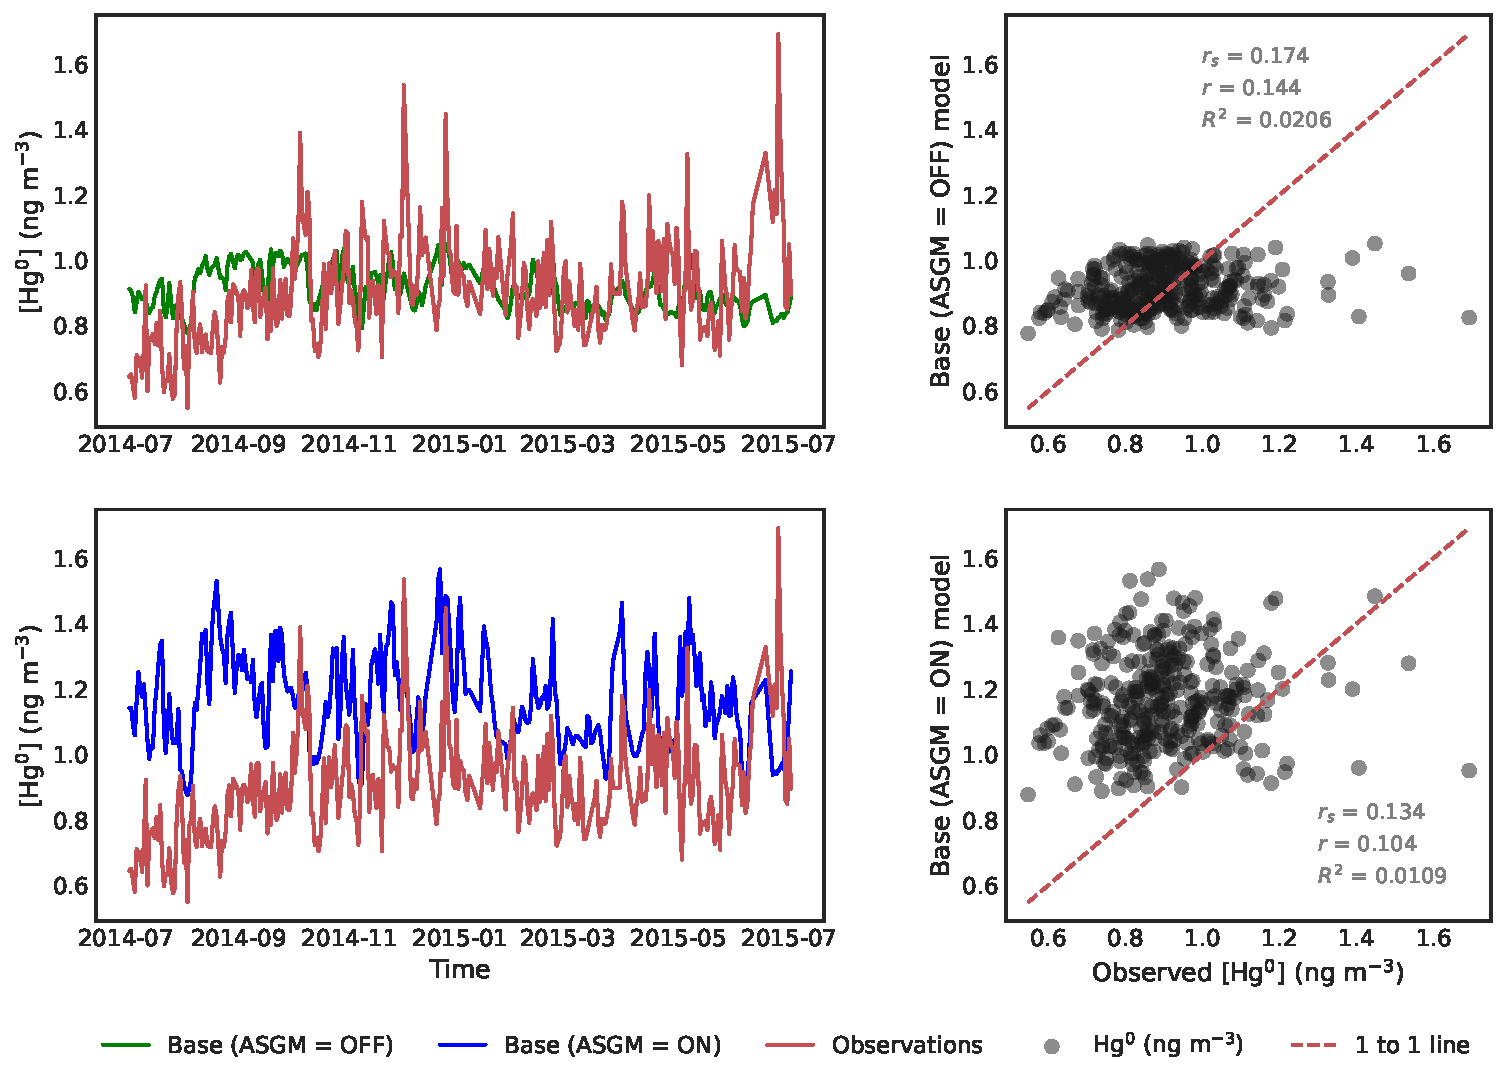
\includegraphics[width=0.85\textwidth]{templates/figures/ModelvsObs/TimeSeriesNsactter_obsVmodel_v1.pdf}
  \centering
  \caption{The observations (in red) are plotted as a function of time in plots (a) and (c) with the \off (in green) in plot (a) and the \on in (blue) in the plot (c). Analysis of the observed Hg concentrations vs. the \off  shows how the modeled mean closely approximates the observed mean and poorly estimates the daily variability, as shown by the difference in the size of the daily spikes of the Hg concentrations. The scatter plots in (b) and (d) represent the modeled \hg  as a function of the measured TGM concentration.}
  \label{fig:ModelvsObsNstats}
\end{figure}
\FloatBarrier

\begin{flushleft}
    Even though GEOS-Chem closely approximated the mean Hg concentrations at CHC in the \off, the Spearman ($r_s$) and Pearson ($r$) correlations between the modeled and observed concentrations were very low at 0.17 and 0.144, respectively. Moreover, the coefficient of determination, $R^2$ between the observed and modeled concentrations in \off case was almost zero at 0.0207. This is in line with the general result in Chapter 2 that the model poorly estimates the observed Hg emission concentrations in the atmosphere. Brasseur and Jacob (p.471 2017) argue that in cases where a model captures the observed means but not the observed variability, the mean may be wrongly interpreted \cite{brasseur_modeling_2017}. Considering this argument in Brasseur and Jacob, the direct comparison of the mean of the \off with the \obsC may be interpreted as wrong because it is known that Hg concentrations in the atmosphere are influenced by ASGM Hg emissions from the ASGM sites near CHC. Furthermore, the model underestimates the observed Hg concentrations due to a poor definition of dry deposition or vegetation uptake.  
\end{flushleft}

\begin{flushleft}
However, the \on reproduces the \iq and 95th \% confidence interval better than it reproduces the mean, as seen in Figure \ref{fig:density_plots_noASGM_vs_ASGM_vsObs}. Density plots of the modeled and observed Hg concentration at Chalcataya are shown in Figure \ref{fig:density_plots_noASGM_vs_ASGM_vsObs}. In (a), the actual distributions for the two simulations and the observations are plotted where the observed TGM concentration distribution is shown in red, the distribution of the \hgc predicted by the \off is shown in green, and that produced by the \on is shown in blue. Figure \ref{fig:density_plots_noASGM_vs_ASGM_vsObs} (b) shows the identical distributions to (a) after standardization by subtracting the mean in each distribution to see how the shapes of the distributions compare with each other.  
\end{flushleft}



\begin{figure}[H]
\begin{tabular}[H]{cc}
\subfloat[]{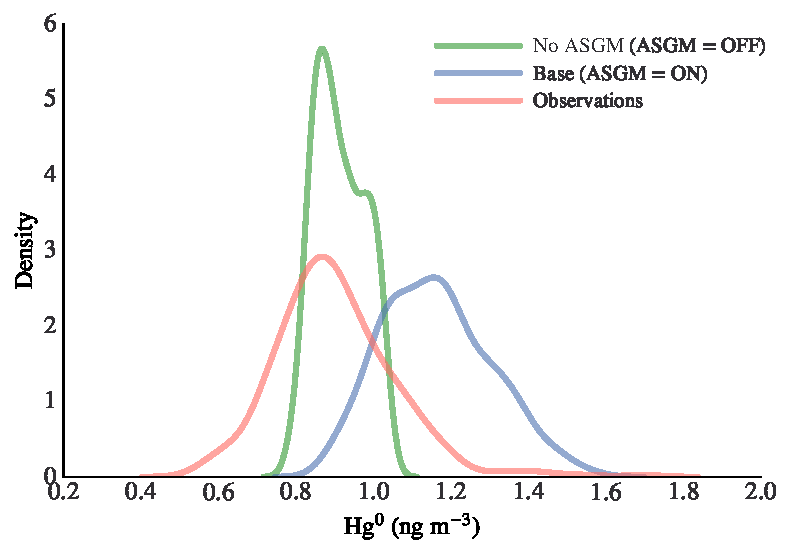
\includegraphics[width = 0.45\linewidth]{templates/figures/ModelvsObs/06-12-22_models_vs_observations_density-plot.pdf}} &
\subfloat[]{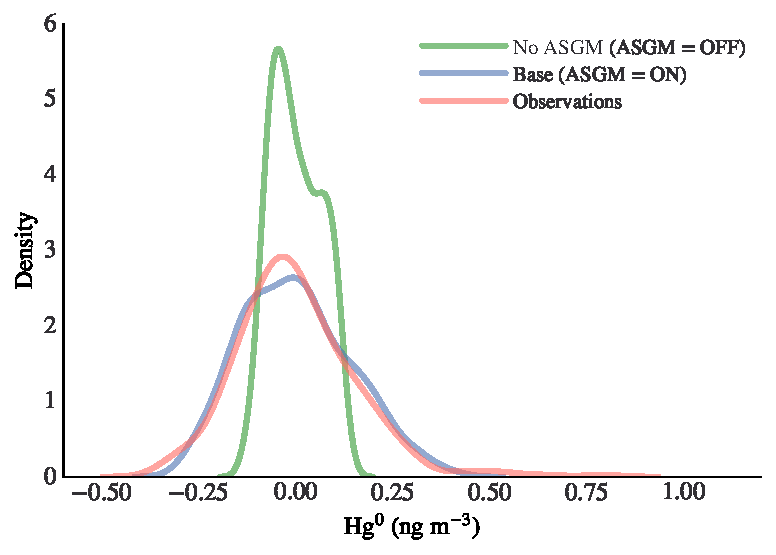
\includegraphics[width = 0.45\linewidth]{templates/figures/ModelvsObs/06-12-22_models_vs_observations_density-plot_std.pdf}}
\end{tabular}
\centering
\captionof{figure}{Density plots of the modeled and observed Hg concentration at Chalcataya. In (a), the actual distributions for the two simulations and the observations are plotted where the observed TGM concentration distribution is shown in red, the distribution of the \hgc predicted by the \off is shown in green, and that produced by the \on is shown in blue. In (b), the same distributions are shown after standardization by subtracting the mean in each distribution for easy comparison of the shapes of the distributions}
\label{fig:density_plots_noASGM_vs_ASGM_vsObs}
\end{figure}
\FloatBarrier
\begin{flushleft}
    Figure \ref{fig:density_plots_noASGM_vs_ASGM_vsObs}, b) shows how the \hgc produced by the \on have a distribution that is similar to the distribution of the observations in terms of standard deviation, \iq and \nft. The \off produced \modelc shows no instance of high \hg concentrations at CHC, and the high concentrations are only produced by the \on. These density plots inform us that the range of observed Hg concentrations in the atmosphere at CHC is primarily influenced by ASGM emissions. Consequently, metrics such as the standard deviation, \iq, and \nft may provide better information about ASGM Hg emission's influence on the observed Hg concentration in the atmosphere than the mean.
\end{flushleft}
\newpage
\subsection{Comparison of Observations with Emission Modification}
\begin{flushleft}
The sensitivity of the modeled \hgc at CHC to the changes in Hg emissions from each grid box in the case study region was investigated by finding the mean, \iq, and correlation as functions of the emissions from each specific grid box.  Figure \ref{fig:mean_of_signals_vs_emissions_per_site} shows the plots of the relationship between the means of \modelc as a function of Hg emissions from the grid box corresponding to the respective regions in the case study. For each plot, the emissions from one grid box are varied while the emissions from the other grid boxes are kept at the level they had in the \on.  The means of \modelc for a given amount of Hg emissions from each grid box are compared to the red horizontal line, which indicates the value of the mean of the observed TGM concentration of 0.90 as presented in Table \ref{tab:ModelvsObsStats}. 
\end{flushleft}

\begin{flushleft}
Moreover, the blue dashed line shows the linear regression line for the values of \modelc as a function of the Hg emissions. All the plots show that the mean of the Hg concentration changes linearly with an increase in emissions and have a $R^2$ value of 1, which validates the linear assumption between emissions and concentrations.
\end{flushleft}
\begin{figure}[H]

\begin{tabular}[H]{cc}
\centering

\subfloat[South Puno]{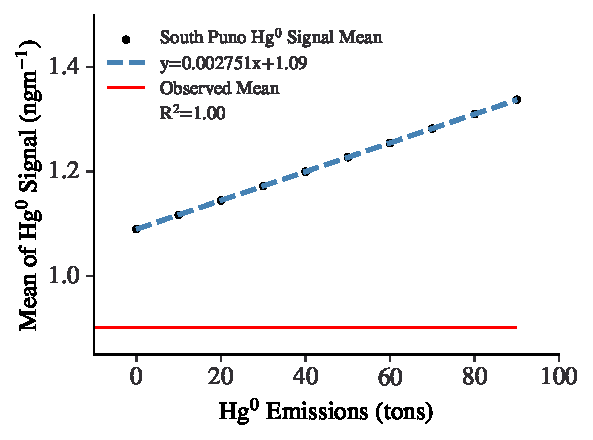
\includegraphics[width = 0.45\linewidth]{templates/figures/individual_site_modifications/mean_Spun_sigs.pdf}} &
\subfloat[North Puno]{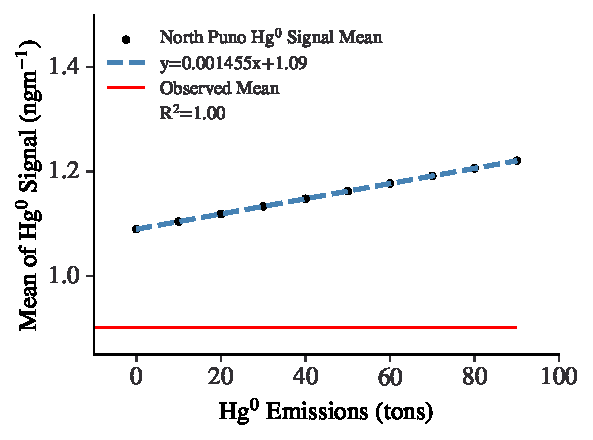
\includegraphics[width = 0.45\linewidth]{templates/figures/individual_site_modifications/mean_Npun_sigs.pdf}}\\
\subfloat[Arequipa]{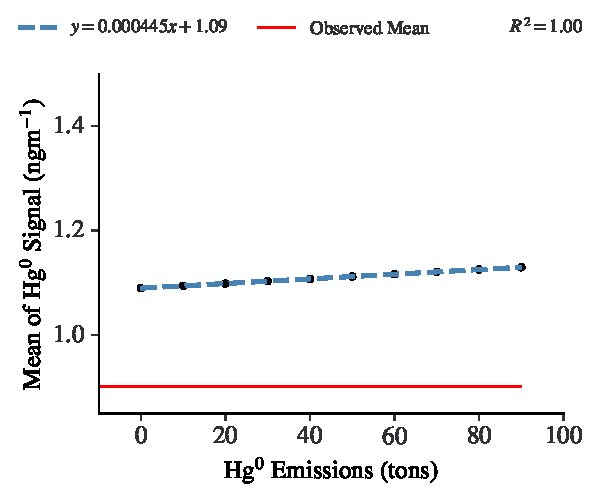
\includegraphics[width = 0.45\linewidth]{templates/figures/individual_site_modifications/mean_Aqp_sigs.pdf}} &
\subfloat[Apurimac]{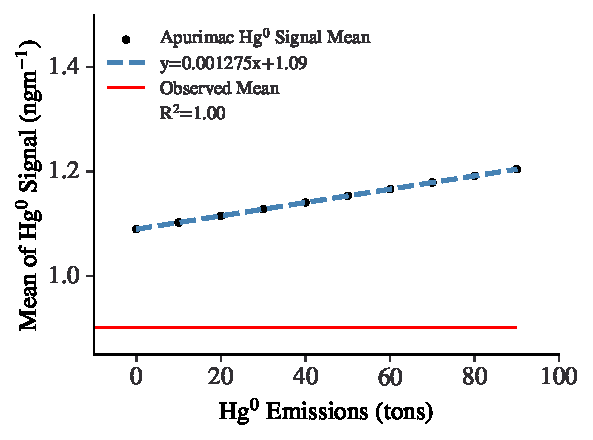
\includegraphics[width = 0.45\linewidth]{templates/figures/individual_site_modifications/mean_Apr_sigs.pdf}}\\
\subfloat[Madre de Dios]{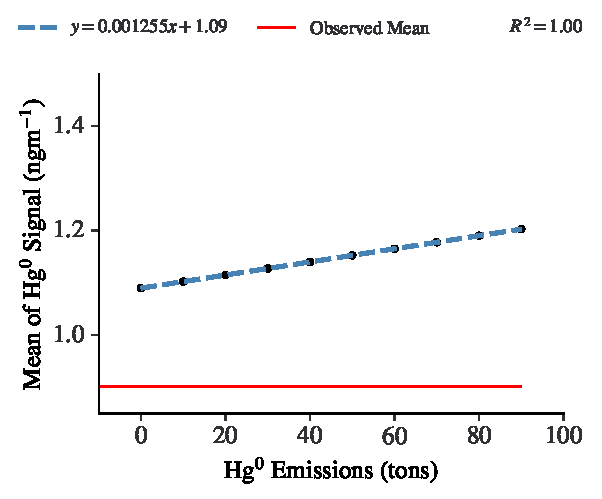
\includegraphics[width = 0.45\linewidth]{templates/figures/individual_site_modifications/mean_Mdd_sigs.pdf}} & \subfloat{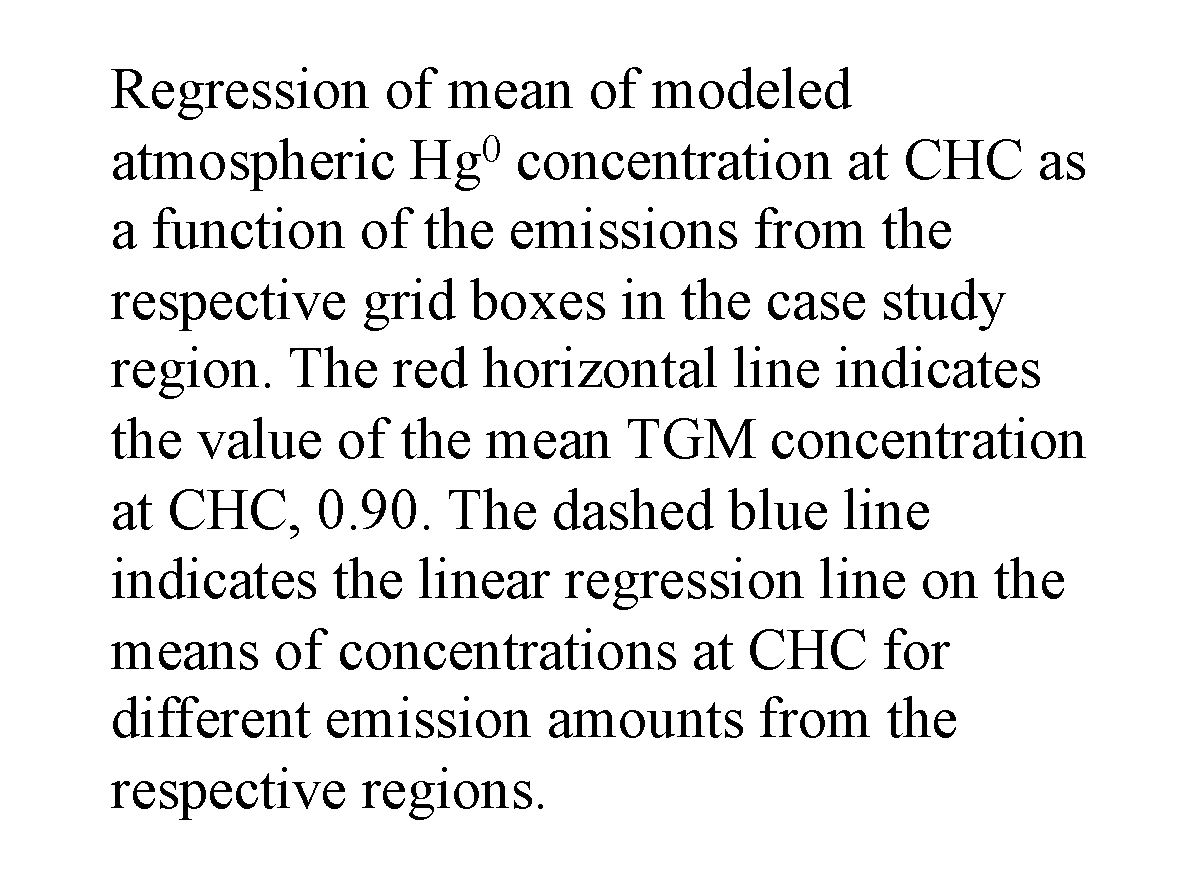
\includegraphics[width = 0.45\linewidth]{templates/figures/individual_site_modifications/mean_caption.pdf}}
\end{tabular}
\caption{ }
\label{fig:mean_of_signals_vs_emissions_per_site}
\end{figure}
\FloatBarrier


\newpage
\begin{flushleft}
    Contrary to Figure \ref{fig:mean_of_signals_vs_emissions_per_site} where the relationships between the Hg emissions and the mean of \modelc have similar \rsq values, the relationship between the \iq of \modelc  and the emissions from each grid box in Figure \ref{fig:iqr_vs_emissions_per_site} have \rsq values that are different. For each plot in Figure \ref{fig:iqr_vs_emissions_per_site}, the emissions from one grid box are varied while the emissions from the other grid boxes are kept at the level they had in the \on. Even though the \rsq values are different, they are all above 0.85, which validates the linear assumption between the emissions and the \rsq values of the Hg concentration. The values of the \iq for a given amount of Hg emissions from each grid box are compared to the red horizontal line, which indicates the \iq of \obsC, 0.16 as presented in Table \ref{tab:ModelvsObsStats}. 
    
\end{flushleft}
\begin{flushleft}
     All the lines showing the relationship between the \iq of \modelc and the emissions intersect the red line representing the \iq of \obsC. The Hg emissions value of the point of intersection between the regression line and the red line can be interpreted as what the emissions from the given grid box should be for the \modelc to match the \obsC. The actual values of the emissions can also be calculated using the regression equation given on each plot. 
     % These estimates are shown in Table \ref{tab:single_site-change_estimates}, and they provide rough constraints on what the emissions from each grid box would have to be for \modelc to match \obsC.
\end{flushleft}

% \begin{flushleft}
%     These estimates are the first ever top-down estimates of Hg emissions from ASGM activities. The top-down estimates mostly agree with the bottom-up estimates from Puno
% \end{flushleft}

%This could be interpreted to means that the emissions from these grid boxes need to be reduced for \modelc to match \obsC. If the relationship between the \iq and emissions depicted in this Figure were to be taken at face value, the emissions from Madre de Dios would have to be 34.18 tonnes. Moreover, the emissions from North Puno would have to be very close to zero, while those from South Puno would have to be about 4 tonnes, and those from Apurimac would have to be about 6 tonnes.  As bottom-up estimates show, reducing emissions from the Madre de Dios region would not be feasible since emissions from Madre de Dios are higher\cite{agc_reporte_2017}. Thus, the intersection of the lines in Figure \ref{fig:iqr_vs_emissions_per_site} with the line representing the observed \iq should not be taken as an indication that emissions from a single source region can lead to a modeled concentration at CHC that matches the observed \iq.
\begin{figure}[H]
\begin{tabular}[H]{cc}
\centering

\subfloat[South Puno]{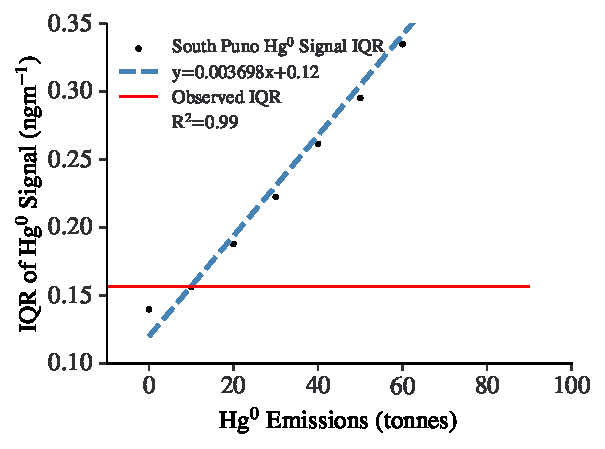
\includegraphics[width = 0.45\linewidth]{templates/figures/individual_site_modifications/iqrSpun_sigs.pdf}} &
\subfloat[North Puno]{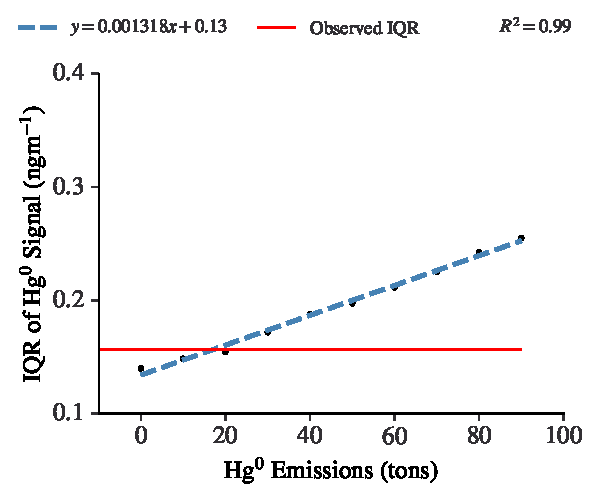
\includegraphics[width = 0.45\linewidth]{templates/figures/individual_site_modifications/iqrNpun_sigs.pdf}}\\
\subfloat[Arequipa]{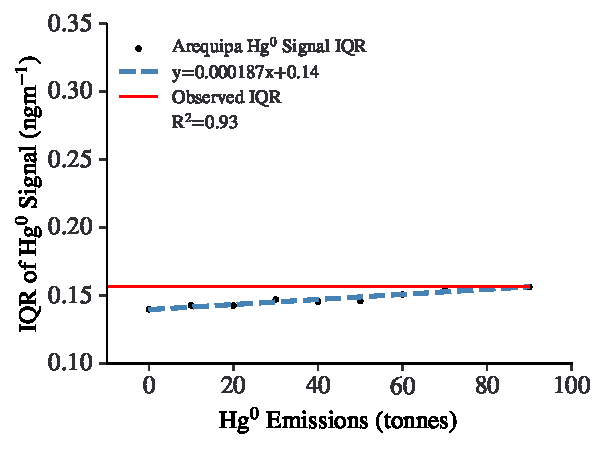
\includegraphics[width = 0.45\linewidth]{templates/figures/individual_site_modifications/iqrAqp_sigs.pdf}} &
\subfloat[Apurimac]{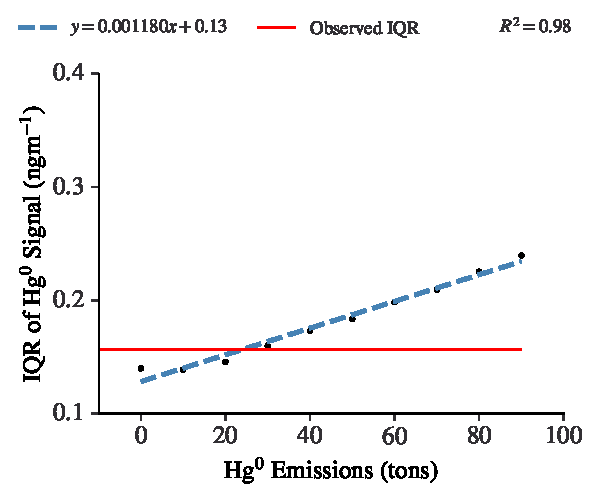
\includegraphics[width = 0.45\linewidth]{templates/figures/individual_site_modifications/iqrApr_sigs.pdf}}\\
\subfloat[Madre de Dios]{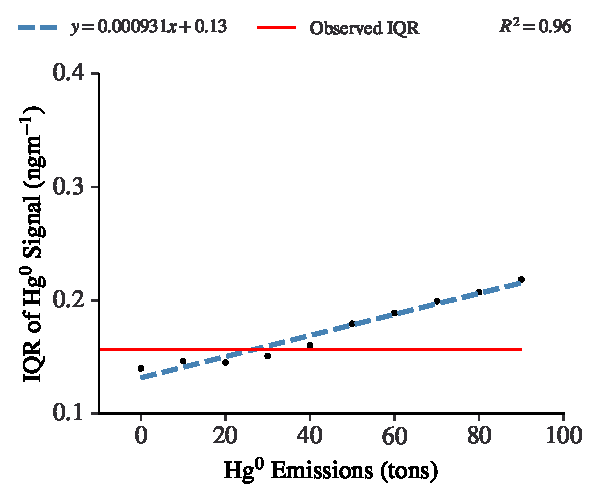
\includegraphics[width = 0.45\linewidth]{templates/figures/individual_site_modifications/iqrMdd_sigs.pdf}} & \subfloat{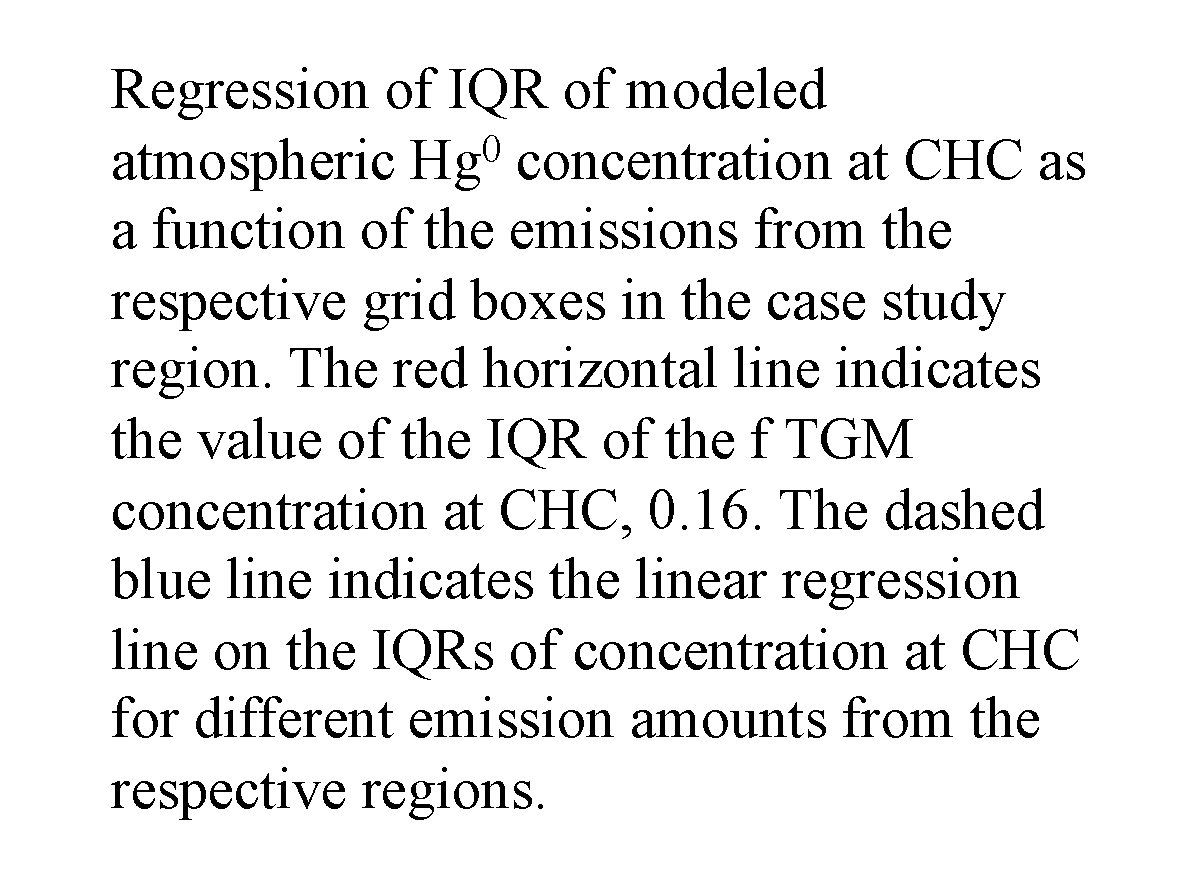
\includegraphics[width = 0.45\linewidth]{templates/figures/individual_site_modifications/iqrcaption.pdf}}
\end{tabular}
\caption{}
\label{fig:iqr_vs_emissions_per_site}
\end{figure}
\FloatBarrier
% \begin{figure}[H]
%   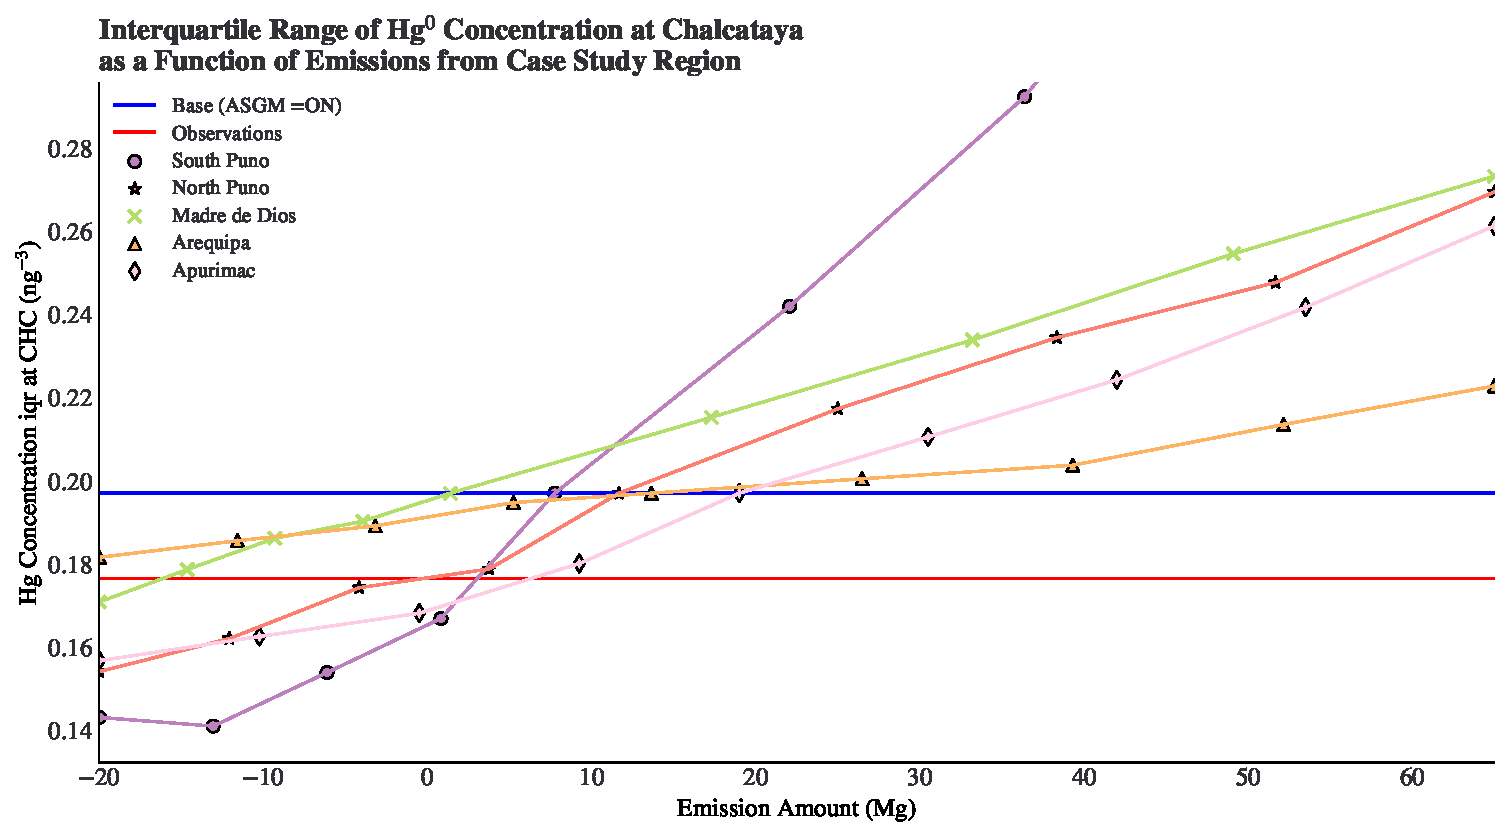
\includegraphics[width=\textwidth]{templates/figures/individual_site_modifications/iqr_vs_emissions.pdf}
%   \centering
%   \caption{ Plot of IQR of \obsC and \modelc as a function of emissions from the case study region. The red horizontal line indicates the observed TGM concentration IQR(0.18). The blue horizontal line indicates the \on predicted \hg IQR. The following shapes show the relationships between the modeled \hg concentration signal IQR at CHC as a function of the emissions from grid boxes in the case study region: South Puno (purple line with circle markers), North Puno (congo pink line with star markers), Madre de Dios (green line with cross markers), Arequipa (orange line with triangle markers), and Apurimac (classic rose line with diamond markers  }
%   \label{fig:iqr_vs_emissions}
% \end{figure}
% \FloatBarrier
\newpage
\begin{flushleft}
     
     Unlike the relationships evident in Figures \ref{fig:mean_of_signals_vs_emissions_per_site} and \ref{fig:iqr_vs_emissions_per_site}, where the relationship between the emissions and the mean or \iq of \modelc is positive, the relationship between the emissions and correlation of \modelc and \obsC shown in Figure \ref{fig:corr_vs_emissions} is negative.  For each plot in Figure \ref{fig:corr_vs_emissions}, the emissions from one grid box are varied while the emissions from the other grid boxes are kept at the level they had in the \on. The red horizontal line indicates the Pearson correlation between \obsC and the \on. The dashed blue line shows the regression line of the correlation between \modelc and \obsC as emissions from each grid box increase. These plots show that it is impossible to improve the Pearson correlation between \modelc and \obsC by changing the emissions.
     
     %The different lines show the correlation between \modelc and \obsC as a function of the emissions from each of the regions: South Puno (purple line with circle markers), North Puno (congo pink line with star markers), Madre de Dios (green line with cross markers), Arequipa (orange line with triangle markers), and Apurimac (classic rose line with diamond markers) The correlation decreases as the emissions from the South Puno, Arequipa, and Apurimac grid boxes increase. 
     
     %These relationships show that changing the emissions from one grid box in the\gc model may not be a reliable way to improve the model's prediction of the observed concentrations, especially because ASGM is no. 

\end{flushleft}


% \begin{figure}[H]
%   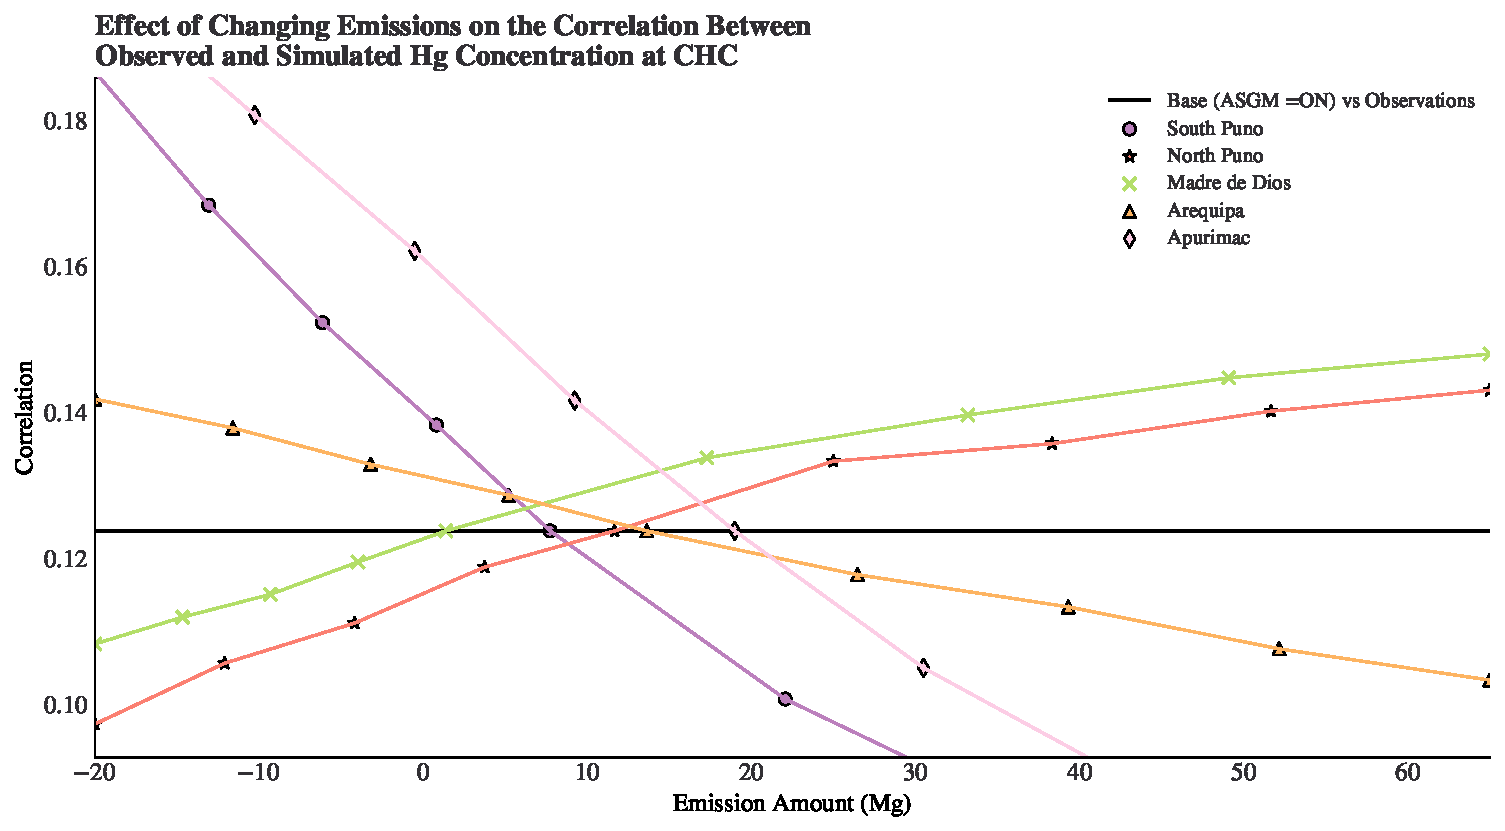
\includegraphics[width=\textwidth]{templates/figures/individual_site_modifications/correlation_vs_emissions.pdf}
%   \centering
%   \caption{Correlation between \obsC and \modelc as a function of emissions from grid boxes associated with the case study region. The black horizontal line indicates the Pearson correlation between \obsC and the \on. The different lines show the correlation between \modelc and \obsC as a function of the emissions from each of the regions: South Puno (purple line with circle markers), North Puno (congo pink line with star markers), Madre de Dios (green line with cross markers), Arequipa (orange line with triangle markers), and Apurimac (classic rose line with diamond markers)}
%   \label{fig:correlation_vs_emissions}
% \end{figure}
% \FloatBarrier
\begin{figure}[H]
\begin{tabular}[H]{cc}
\centering

\subfloat[South Puno]{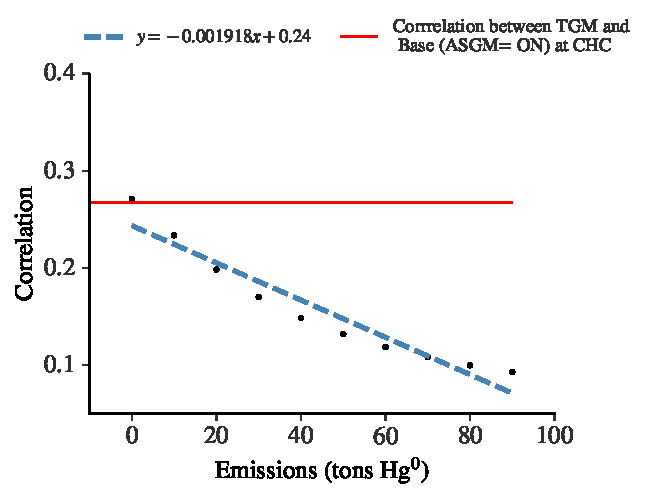
\includegraphics[width = 0.45\linewidth]{templates/figures/individual_site_modifications/corr_Spun_sigs.pdf}} &
\subfloat[North Puno]{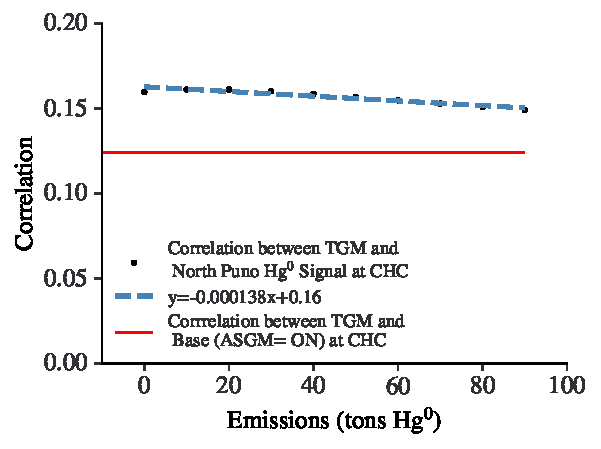
\includegraphics[width = 0.45\linewidth]{templates/figures/individual_site_modifications/corr_Npun_sigs.pdf}}\\
\subfloat[Arequipa]{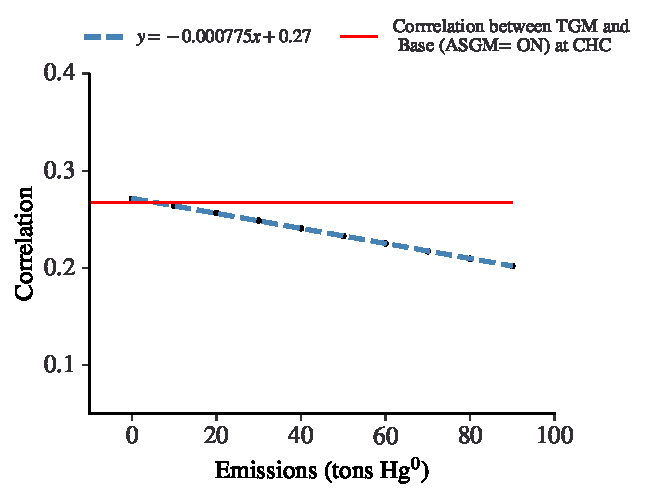
\includegraphics[width = 0.45\linewidth]{templates/figures/individual_site_modifications/corr_Aqp_sigs.pdf}} &
\subfloat[Apurimac]{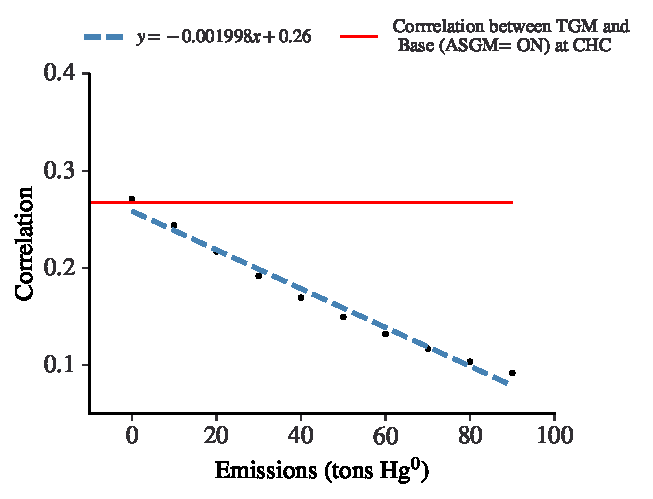
\includegraphics[width = 0.45\linewidth]{templates/figures/individual_site_modifications/corr_Apr_sigs.pdf}}\\
\subfloat[Madre de Dios]{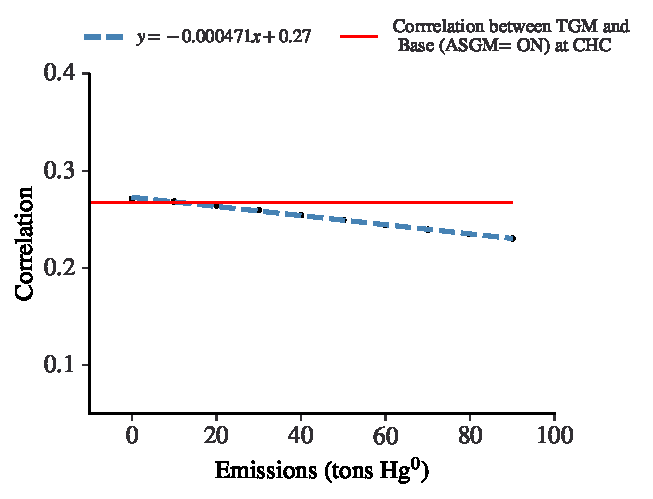
\includegraphics[width = 0.45\linewidth]{templates/figures/individual_site_modifications/corr_Mdd_sigs.pdf}} & \subfloat{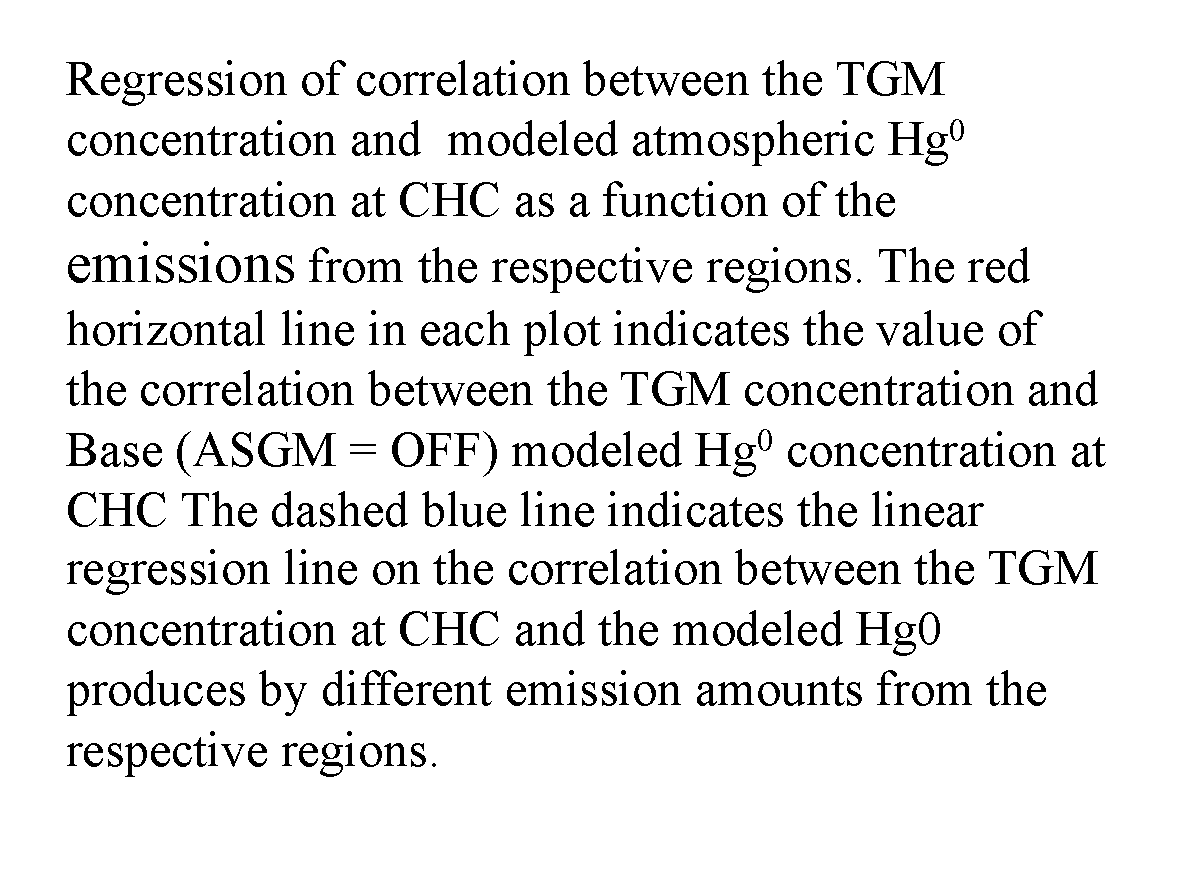
\includegraphics[width = 0.45\linewidth]{templates/figures/individual_site_modifications/corr_caption.pdf}}
\end{tabular}
\caption{ }
\label{fig:corr_vs_emissions}
\end{figure}
\FloatBarrier

\newpage
% \begin{table}[H]
% \caption{Table showing the emission estimates for each of the grid boxes in the case study region when the \iq is used as the metric to compare \modelc to \obsC after modifying emissions from one site and when the \nft is used}
%     \label{tab:single_site-change_estimates}
% \begin{tabular}{lcc}

% \textbf{Region}        & \textbf{Emission Estimate }        &  \textbf{Emission Estimate }\\
%                         &  \iq (tonnes)       &   \nft (tonnes) \\
% \hline
% Madre de Dios          & $26.82$                                    & $78.10$ \\

% North Puno             & $17.16$                                   & $24.87$  \\
        
% South Puno             & $9.93$                                    & $59.46$   \\

% Apurimac               & $24.08$                                   & $62.86$  \\

% Arequipa               & $90.77$                                   & $178.45$  \\


% \hline
% \end{tabular}
% \centering
% \end{table}
\begin{flushleft}
     This section has shown the effect of changing Hg emissions from individual grid boxes on the modeled \hgc at a distant active monitoring site like CHC. The \iq and \nft produced some estimates of the \hg emissions from the different regions. However, the range of these estimates is not within the estimates discussed in  section 3.3.1. These estimates were more informative about the potential constraints on the emissions from the region. The following section presents the emission estimates generated using the MCMC to investigate the effect of changing emissions from multiple sites instead of changing the emissions from one site as discussed in this section.  
     
     %Other processes, such as vegetation uptake, have been shown to impact the amount of Hg in the atmosphere, and Feinberg et al 2022 showed that this version of \gc had a poor representation of vegetation uptake\cite{feinberg_evaluating_2022}.  Furthermore, comparing the Peru national inventory of emissions developed by the AGC\cite{agc_reporte_2017} and the global inventory in the GMA 2018\cite{steenhuisen_development_2019,united_nations_environment_programme_technical_2019} as we did in section 3.3.1 shows that there are numerous mismatches between the actual emissions and the emissions used by \gc to simulate the \hgc in the atmosphere.

   
 
\end{flushleft}

\subsection{Estimating Emissions with Markov Chain Monte Carlo}
The MCMC approach produced \hg emissions estimates within the ranges of estimates produced by the bottom-up inventories when the \nft was used to compare \obsC to \modelc. Figure \ref{fig:MCMC_estimates95th} show's the distributions of the estimates produced by the MCMC approach. The \hg emission estimates when the \nft is used as the metric to compare \modelc, and \obsC is shown by the box and whisker plots. The horizontal lines representing the emission estimates from the bottom-up inventories are traced over the box plots. The solid horizontal lines represent the emission estimates from the GMA 2018 inventory \cite{united_nations_environment_programme_technical_2019,steenhuisen_development_2019} and the dashed lines represent the emission estimates from the bottom-up inventory published by the Artisanal Gold Counsel\cite{agc_reporte_2017}. The estimated values and ranges of emissions are detailed in Table \ref{tab:MCMC_estimates}. 
\begin{figure}[H]
  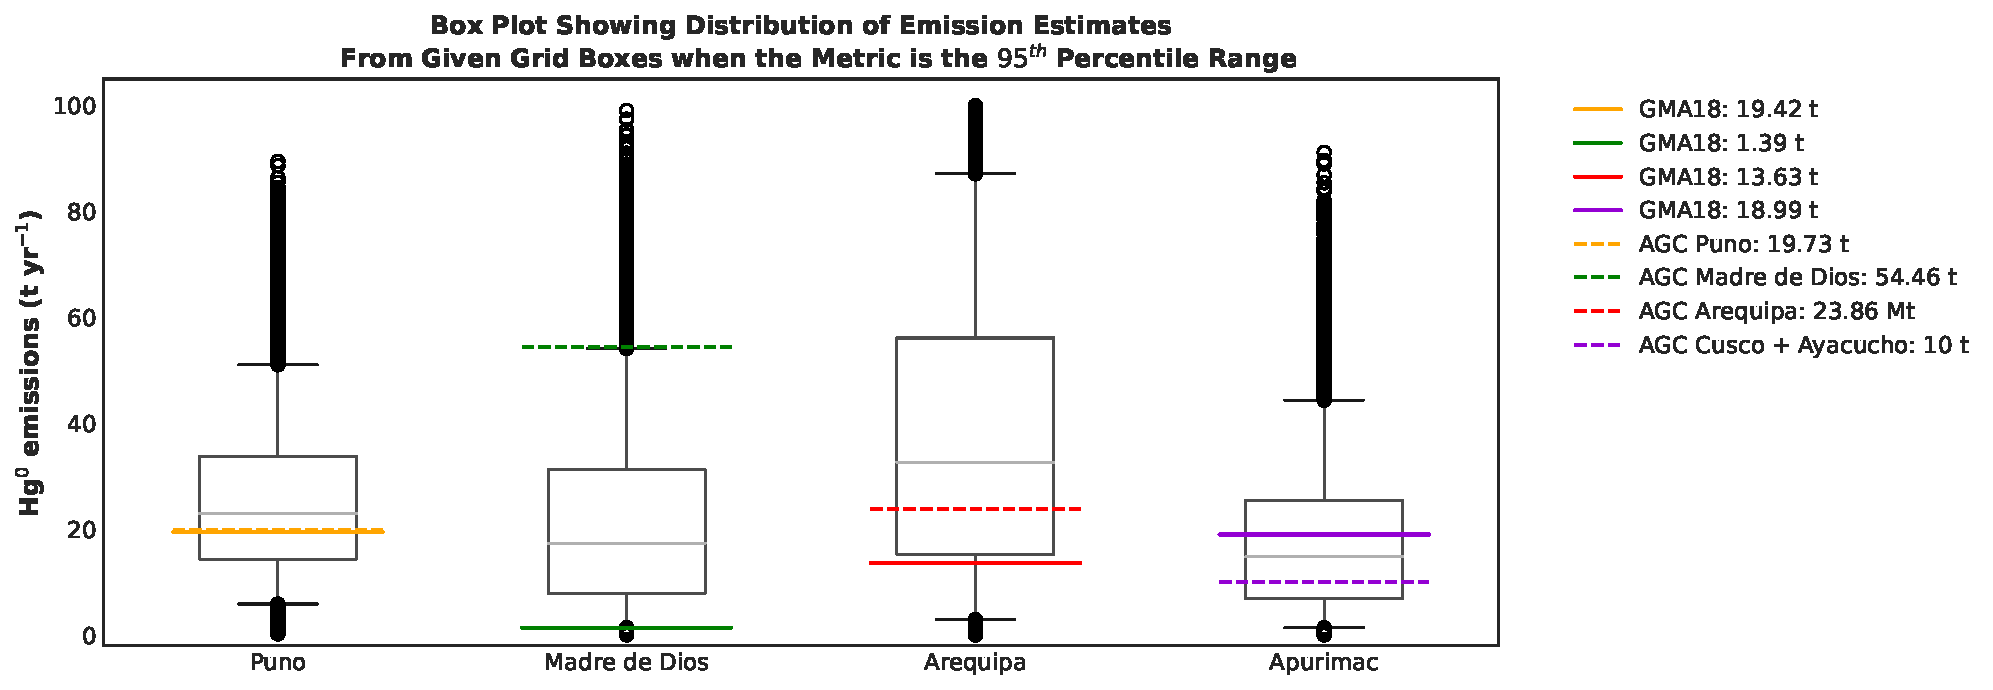
\includegraphics[width=\textwidth]{templates/figures/MCMC/MCMCMCMC_Estimates95th.pdf}
  \centering
  \caption{Emission Estimates when the $95^{th}$ percentile range is used as the metric to compare the model outputs to observations. The horizontal lines representing the emission estimates from the bottom-up inventories are traced over the box plots. The solid horizontal lines represent the emission estimates from the GMA 2018 inventory \cite{united_nations_environment_programme_technical_2019,steenhuisen_development_2019} and the dashed lines represent the emission estimates from the bottom-up inventory published by the Artisanal Gold Counsel\cite{agc_reporte_2017}.}
  \label{fig:MCMC_estimates95th}
\end{figure}
\FloatBarrier
% % \renewcommand{\arraystretch}{2}
% \begin{flushleft}
%      The mean was the worst metric to use in the MCMC to reproduce the GMA 2018 emissions estimates, while the \nft reproduced the GMA 2018 emissions estimates with the least absolute error, followed by the \iq. This further corroborated the earlier finding that the mean was not a reliable metric, in this case, to compare the observed Hg concentration in the atmosphere to the modeled \hg concentrations.
% \end{flushleft}

%      Figure \ref{fig:MCMC_emetrics} compares the absolute error of different metrics when used in the MCMC to generate estimates of the emissions from different departments in Peru. The absolute error is a function of the type of metric used. The plus signs show the absolute error in reproducing emissions from the case study region(Puno (blue), Madre de Dios (orange), Arequipa (green), and Apurimac (red)) for each metric.

% \begin{figure}[H]
%   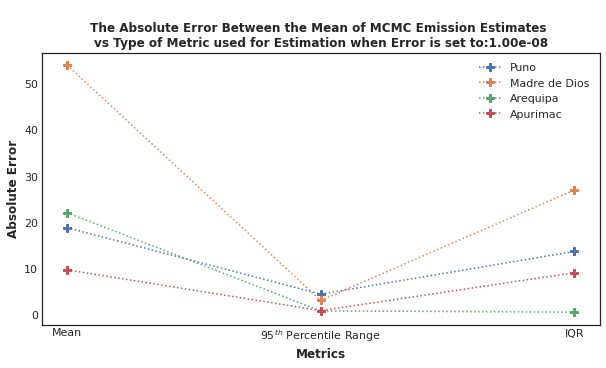
\includegraphics[width=\textwidth]{templates/figures/MCMC/comparison of matrics.png}
%   \centering
%   \caption{Comparison of the absolute error of different metrics when used in the MCMC to generate estimates of the emissions from different grid boxes in the case study region. The Absolute error is a function of the type of metric used. The plus signs show the absolute error in reproducing emissions from the case study region(Puno (blue), Madre de Dios (orange), Arequipa (green), and Apurimac (red)) for each metric.  }
%   \label{fig:MCMC_emetrics}
% \end{figure}
% \FloatBarrier
\begin{flushleft}
    These estimates are the first ever top-down estimates of Hg emissions from ASGM activities. It is critical to note that the ranges of the estimates are huge. Therefore, these results may be improved if more data from monitoring sites were available to constrain the emissions. 
\end{flushleft}    
\begin{table}[H]
\caption{Table showing the emission estimates for each of the grid boxes in the case study region when the $95^{th}$ percentile range is used as the metric to compare the model outputs to observations}
    \label{tab:MCMC_estimates}
\begin{tabular}{lcc}

\textbf{Region}        & \textbf{Emission Estimate (Mg)}  &     \textbf{Range of Estimate (Mg)}                      \\
\hline
Madre de Dios          & $21$                               & $1.36 - 54.12$\\

Apurimac               & $17$                               & $1.36 - 44.37$\\

Arequipa               & $37$                               & $2.88 - 87.14$\\

Puno                    & $25$                              & $5.85 - 51.05$\\
\hline
Total                  & $101$                            &  $11.45 - 236.69$ \\
\hline
\end{tabular}
\centering
\end{table}

\begin{flushleft}
 % I argued that poor parameterization of dry deposition in \gcs version 12.8.1 might be one of the reasons for this poor performance of the model in reproducing the mean of \obsC. Moreover, this phenomenon was investigated and addressed for future \gc versions in Feinberg et al (2022). I also hypothesized that the model poorly predicted Hg concentrations in the atmosphere because of faults in the emission estimates used in the model. 
  We produced top-down estimates of the corresponding emissions for four Peruvian departments in the case study region. The estimated emissions and the ranges are shown in Table \ref{tab:MCMC_estimates} resulting in 101.23 tonnes of emissions from Peru per year, ranging from 11.45 tonnes to 236.69 tonnes. This is a wide range, but it's a confidence interval based on the data and model uncertainty discussed so far. The proof of concept I developed shows that even with a minimal data set and an uncertain model, we can calculate top-down estimates of ASGM \hg emissions. Improved parameterization of vegetation uptake may help narrow the vast uncertainty ranges in the emission estimates produced by this approach and improve confidence in the \hg emission estimates. However, significant improvements will be realized if more relevant measurements of atmospheric Hg are used instead of one-site data as we did in this analysis.  
  \end{flushleft}
  
  \begin{flushleft}
  Such model improvements are discussed in Feinberg et al.(2022)\cite{feinberg_evaluating_2022} and may enable the use of the mean as a metric for producing the \hg emission estimates, which we could not not use in this analysis. Additional data is another essential source of improvement, particularly time series data rather than annual averages as I have shown by using different time periods from \obsC dataset. Moreover, these results demonstrate that for non-point sources, such as ASGM, where the variability over time is somewhat unpredictable, extreme values provide vital information for source quantification. The analysis in this chapter focused on a region in Peru, where ASGM dominates to use top-down techniques for quantifying ASGM Hg emissions. Implementing this approach will be challenging in areas where ASGM occurs concurrently with many point sources, such as Southeast Asia, where biomass burning and coal combustion. For Hg monitoring sites in mountainous regions such as CHC, the global scale resolution of GEOS-Chem is not particularly suitable. Therefore, future work may extend this method and this proof of concept using finer resolutions with a regional focus.
   \end{flushleft}
  
  \begin{flushleft}
  A further benefit of the above analysis is that it helps address this thesis's first about how regional atmospheric modeling and monitoring can help reconcile the differences in global and national emission estimates. The produced emissions estimates were within the bounds of the national and global inventories, and having more observation site data would help bolster the credibility of the estimates. Moreover, the about analysis bolsters the answers to this thesis's second question in Chapter 2 about how regional monitring networks can improve the utility of models for the effectiveness evaluation of the MC. The active monitoring data from the CHC GMOS site was used to generate emission estimates for distant regions. These inverse modeling approaches would be hard to implement with the PAS data, but the active sampling data was amenable to dissection in different summary metrics such as the mean, \iq, correlation, and the \nft. Even though the mean was not viable for this analysis, the other metrics were instrumental in the result. This kind of breakdown of the observed emissions may not be possible with the PAS data.
\end{flushleft}

% \begin{figure}[H]
%   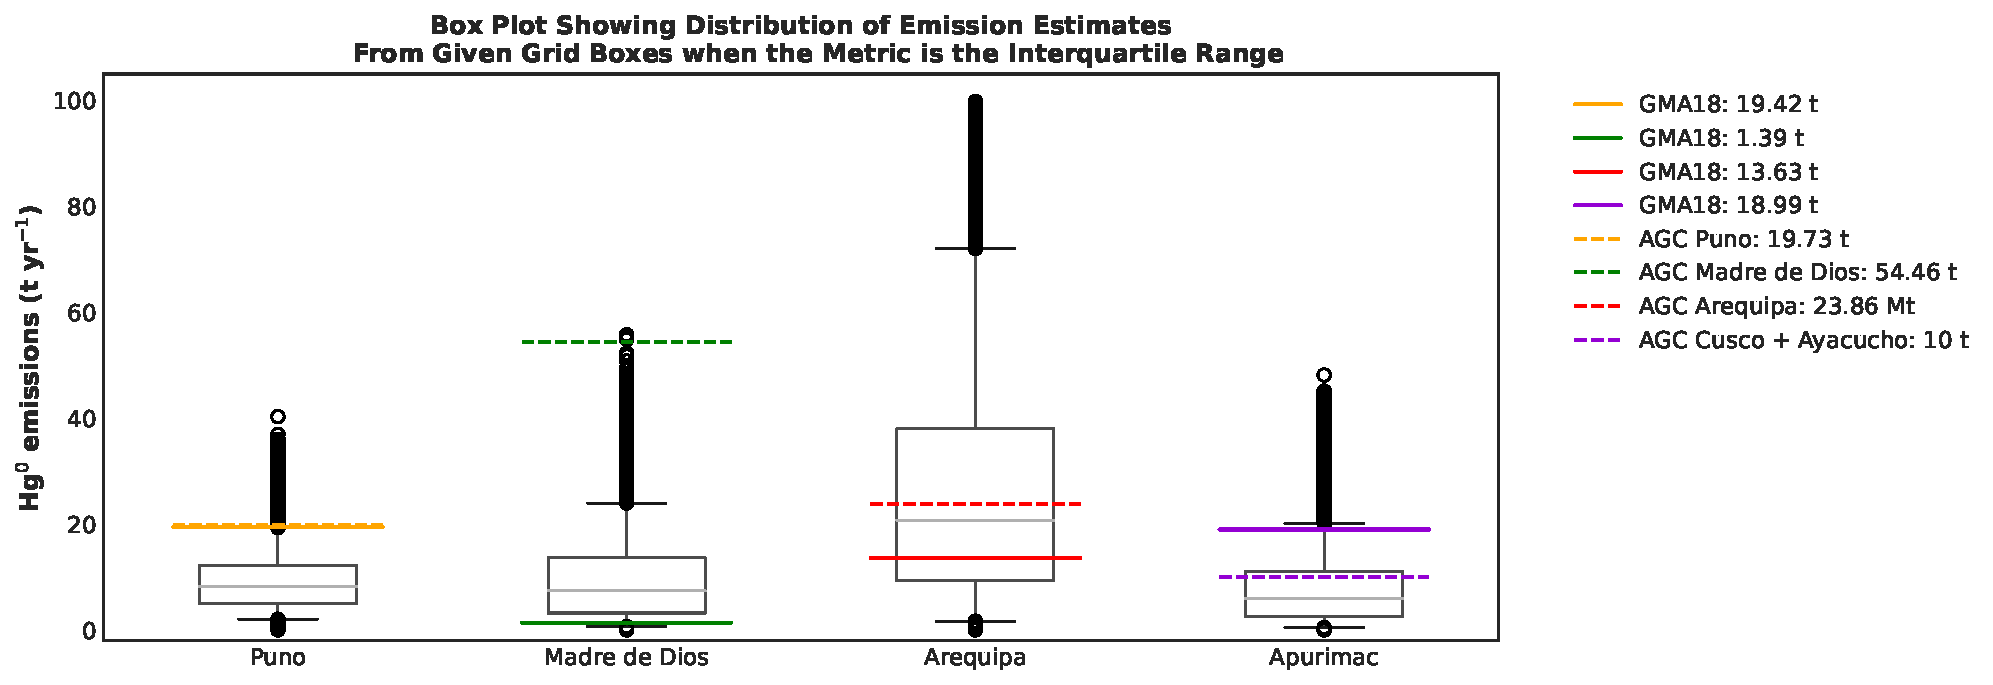
\includegraphics[width=\textwidth]{templates/figures/MCMC/MCMCMCMC_Estimatesiqr.pdf}
%   \centering
%   \caption{Emission Estimates when the \iq is used as the metric to compare the model outputs to observations. The horizontal lines representing the emission estimates from the bottom-up inventories are traced over the box plots. The solid horizontal lines represent the emission estimates from the GMA 2018 inventory \cite{united_nations_environment_programme_technical_2019,steenhuisen_development_2019} and the dashed lines represent the emission estimates from the bottom-up inventory published by the Artisanal Gold Counsel\cite{agc_reporte_2017}.}
%   \label{fig:MCMC_estimates95}
% \end{figure}
% \FloatBarrier
\newpage
\section{Conclusion}
\begin{flushleft}
In this study, I demonstrate how top-down estimates of Hg emissions from ASGM activities can be generated using a CTM and time series monitoring data. Limited data sources and uncertain models prevented precise calculations, but the emissions were within the ranges estimated by the GMA 2018\cite{steenhuisen_development_2019,united_nations_environment_programme_technical_2019} and the Artisanal Gold Council\cite{agc_reporte_2017}. By defining vegetation uptake better, the model improvements discussed in Feinberg et al. (2022) will improve this approach and potentially increase the utility of mean concentrations as a viable metric to use in the analysis\cite{feinberg_evaluating_2022}. Additionally, more time series data will enhance the accuracy and credibility of the model's estimates. Given future work and interest in applying this method in other regions, I noted that this approach was applied to a case study region in Latin America, where ASGM is the dominant source. It may be challenging to extend this approach to areas where ASGM Hg emissions occur in tandem with other emission sources.
 
\end{flushleft}
